\documentclass[1p]{elsarticle_modified}
%\bibliographystyle{elsarticle-num}

%\usepackage[colorlinks]{hyperref}
%\usepackage{abbrmath_seonhwa} %\Abb, \Ascr, \Acal ,\Abf, \Afrak
\usepackage{amsfonts}
\usepackage{amssymb}
\usepackage{amsmath}
\usepackage{amsthm}
\usepackage{scalefnt}
\usepackage{amsbsy}
\usepackage{kotex}
\usepackage{caption}
\usepackage{subfig}
\usepackage{color}
\usepackage{graphicx}
\usepackage{xcolor} %% white, black, red, green, blue, cyan, magenta, yellow
\usepackage{float}
\usepackage{setspace}
\usepackage{hyperref}

\usepackage{tikz}
\usetikzlibrary{arrows}

\usepackage{multirow}
\usepackage{array} % fixed length table
\usepackage{hhline}

%%%%%%%%%%%%%%%%%%%%%
\makeatletter
\renewcommand*\env@matrix[1][\arraystretch]{%
	\edef\arraystretch{#1}%
	\hskip -\arraycolsep
	\let\@ifnextchar\new@ifnextchar
	\array{*\c@MaxMatrixCols c}}
\makeatother %https://tex.stackexchange.com/questions/14071/how-can-i-increase-the-line-spacing-in-a-matrix
%%%%%%%%%%%%%%%

\usepackage[normalem]{ulem}

\newcommand{\msout}[1]{\ifmmode\text{\sout{\ensuremath{#1}}}\else\sout{#1}\fi}
%SOURCE: \msout is \stkout macro in https://tex.stackexchange.com/questions/20609/strikeout-in-math-mode

\newcommand{\cancel}[1]{
	\ifmmode
	{\color{red}\msout{#1}}
	\else
	{\color{red}\sout{#1}}
	\fi
}

\newcommand{\add}[1]{
	{\color{blue}\uwave{#1}}
}

\newcommand{\replace}[2]{
	\ifmmode
	{\color{red}\msout{#1}}{\color{blue}\uwave{#2}}
	\else
	{\color{red}\sout{#1}}{\color{blue}\uwave{#2}}
	\fi
}

\newcommand{\Sol}{\mathcal{S}} %segment
\newcommand{\D}{D} %diagram
\newcommand{\A}{\mathcal{A}} %arc


%%%%%%%%%%%%%%%%%%%%%%%%%%%%%5 test

\def\sl{\operatorname{\textup{SL}}(2,\Cbb)}
\def\psl{\operatorname{\textup{PSL}}(2,\Cbb)}
\def\quan{\mkern 1mu \triangleright \mkern 1mu}

\theoremstyle{definition}
\newtheorem{thm}{Theorem}[section]
\newtheorem{prop}[thm]{Proposition}
\newtheorem{lem}[thm]{Lemma}
\newtheorem{ques}[thm]{Question}
\newtheorem{cor}[thm]{Corollary}
\newtheorem{defn}[thm]{Definition}
\newtheorem{exam}[thm]{Example}
\newtheorem{rmk}[thm]{Remark}
\newtheorem{alg}[thm]{Algorithm}

\newcommand{\I}{\sqrt{-1}}
\begin{document}

%\begin{frontmatter}
%
%\title{Boundary parabolic representations of knots up to 8 crossings}
%
%%% Group authors per affiliation:
%\author{Yunhi Cho} 
%\address{Department of Mathematics, University of Seoul, Seoul, Korea}
%\ead{yhcho@uos.ac.kr}
%
%
%\author{Seonhwa Kim} %\fnref{s_kim}}
%\address{Center for Geometry and Physics, Institute for Basic Science, Pohang, 37673, Korea}
%\ead{ryeona17@ibs.re.kr}
%
%\author{Hyuk Kim}
%\address{Department of Mathematical Sciences, Seoul National University, Seoul 08826, Korea}
%\ead{hyukkim@snu.ac.kr}
%
%\author{Seokbeom Yoon}
%\address{Department of Mathematical Sciences, Seoul National University, Seoul, 08826,  Korea}
%\ead{sbyoon15@snu.ac.kr}
%
%\begin{abstract}
%We find all boundary parabolic representation of knots up to 8 crossings.
%
%\end{abstract}
%\begin{keyword}
%    \MSC[2010] 57M25 
%\end{keyword}
%
%\end{frontmatter}

%\linenumbers
%\tableofcontents
%
\newcommand\colored[1]{\textcolor{white}{\rule[-0.35ex]{0.8em}{1.4ex}}\kern-0.8em\color{red} #1}%
%\newcommand\colored[1]{\textcolor{white}{ #1}\kern-2.17ex	\textcolor{white}{ #1}\kern-1.81ex	\textcolor{white}{ #1}\kern-2.15ex\color{red}#1	}

{\Large $\underline{12a_{0875}~(K12a_{0875})}$}

\setlength{\tabcolsep}{10pt}
\renewcommand{\arraystretch}{1.6}
\vspace{1cm}\begin{tabular}{m{100pt}>{\centering\arraybackslash}m{274pt}}
\multirow{5}{120pt}{
	\centering
	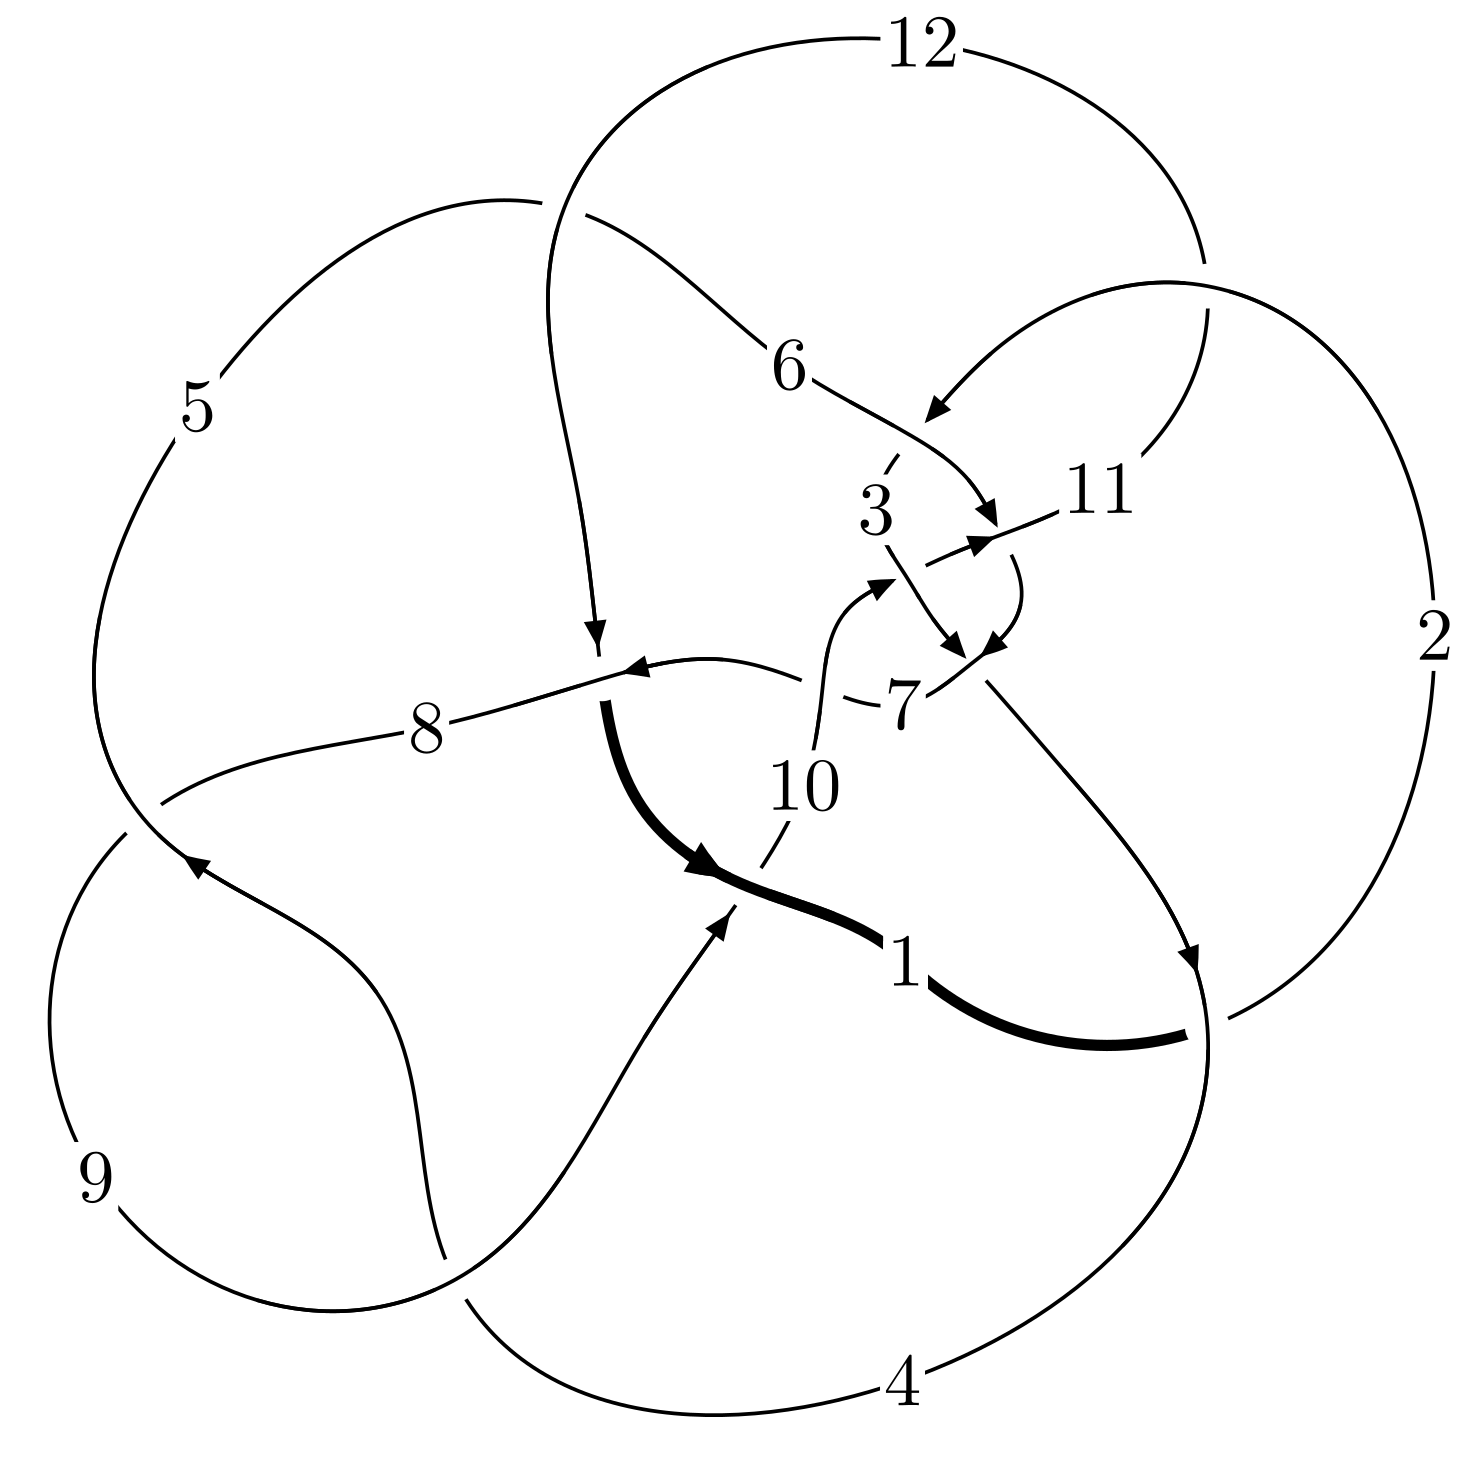
\includegraphics[width=112pt]{../../../GIT/diagram.site/Diagrams/png/1676_12a_0875.png}\\
\ \ \ A knot diagram\footnotemark}&
\allowdisplaybreaks
\textbf{Linearized knot diagam} \\
\cline{2-2}
 &
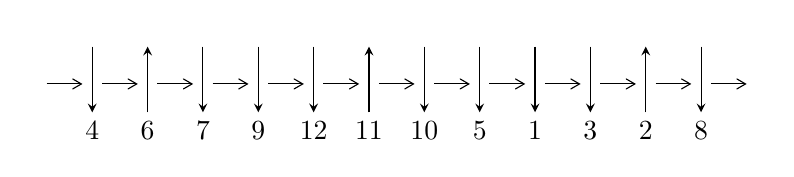
\begin{tikzpicture}[x=20pt, y=17pt]
	% nodes
	\node (C0) at (0, 0) {};
	\node (C1) at (1, 0) {};
	\node (C1U) at (1, +1) {};
	\node (C1D) at (1, -1) {4};

	\node (C2) at (2, 0) {};
	\node (C2U) at (2, +1) {};
	\node (C2D) at (2, -1) {6};

	\node (C3) at (3, 0) {};
	\node (C3U) at (3, +1) {};
	\node (C3D) at (3, -1) {7};

	\node (C4) at (4, 0) {};
	\node (C4U) at (4, +1) {};
	\node (C4D) at (4, -1) {9};

	\node (C5) at (5, 0) {};
	\node (C5U) at (5, +1) {};
	\node (C5D) at (5, -1) {12};

	\node (C6) at (6, 0) {};
	\node (C6U) at (6, +1) {};
	\node (C6D) at (6, -1) {11};

	\node (C7) at (7, 0) {};
	\node (C7U) at (7, +1) {};
	\node (C7D) at (7, -1) {10};

	\node (C8) at (8, 0) {};
	\node (C8U) at (8, +1) {};
	\node (C8D) at (8, -1) {5};

	\node (C9) at (9, 0) {};
	\node (C9U) at (9, +1) {};
	\node (C9D) at (9, -1) {1};

	\node (C10) at (10, 0) {};
	\node (C10U) at (10, +1) {};
	\node (C10D) at (10, -1) {3};

	\node (C11) at (11, 0) {};
	\node (C11U) at (11, +1) {};
	\node (C11D) at (11, -1) {2};

	\node (C12) at (12, 0) {};
	\node (C12U) at (12, +1) {};
	\node (C12D) at (12, -1) {8};
	\node (C13) at (13, 0) {};

	% arrows
	\draw[->,>={angle 60}]
	(C0) edge (C1) (C1) edge (C2) (C2) edge (C3) (C3) edge (C4) (C4) edge (C5) (C5) edge (C6) (C6) edge (C7) (C7) edge (C8) (C8) edge (C9) (C9) edge (C10) (C10) edge (C11) (C11) edge (C12) (C12) edge (C13) ;	\draw[->,>=stealth]
	(C1U) edge (C1D) (C2D) edge (C2U) (C3U) edge (C3D) (C4U) edge (C4D) (C5U) edge (C5D) (C6D) edge (C6U) (C7U) edge (C7D) (C8U) edge (C8D) (C9U) edge (C9D) (C10U) edge (C10D) (C11D) edge (C11U) (C12U) edge (C12D) ;
	\end{tikzpicture} \\
\hhline{~~} \\& 
\textbf{Solving Sequence} \\ \cline{2-2} 
 &
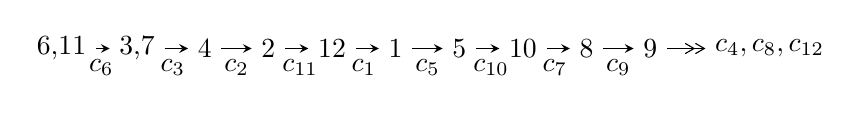
\begin{tikzpicture}[x=23pt, y=7pt]
	% node
	\node (A0) at (-1/8, 0) {6,11};
	\node (A1) at (17/16, 0) {3,7};
	\node (A2) at (17/8, 0) {4};
	\node (A3) at (25/8, 0) {2};
	\node (A4) at (33/8, 0) {12};
	\node (A5) at (41/8, 0) {1};
	\node (A6) at (49/8, 0) {5};
	\node (A7) at (57/8, 0) {10};
	\node (A8) at (65/8, 0) {8};
	\node (A9) at (73/8, 0) {9};
	\node (C1) at (1/2, -1) {$c_{6}$};
	\node (C2) at (13/8, -1) {$c_{3}$};
	\node (C3) at (21/8, -1) {$c_{2}$};
	\node (C4) at (29/8, -1) {$c_{11}$};
	\node (C5) at (37/8, -1) {$c_{1}$};
	\node (C6) at (45/8, -1) {$c_{5}$};
	\node (C7) at (53/8, -1) {$c_{10}$};
	\node (C8) at (61/8, -1) {$c_{7}$};
	\node (C9) at (69/8, -1) {$c_{9}$};
	\node (A10) at (11, 0) {$c_{4},c_{8},c_{12}$};

	% edge
	\draw[->,>=stealth]	
	(A0) edge (A1) (A1) edge (A2) (A2) edge (A3) (A3) edge (A4) (A4) edge (A5) (A5) edge (A6) (A6) edge (A7) (A7) edge (A8) (A8) edge (A9) ;
	\draw[->>,>={angle 60}]	
	(A9) edge (A10);
\end{tikzpicture} \\ 

\end{tabular} \\

\footnotetext{
The image of knot diagram is generated by the software ``\textbf{Draw programme}" developed by Andrew Bartholomew(\url{http://www.layer8.co.uk/maths/draw/index.htm\#Running-draw}), where we modified some parts for our purpose(\url{https://github.com/CATsTAILs/LinksPainter}).
}\phantom \\ \newline 
\centering \textbf{Ideals for irreducible components\footnotemark of $X_{\text{par}}$} 
 
\begin{align*}
I^u_{1}&=\langle 
6.06777\times10^{2287} u^{207}+3.61028\times10^{2288} u^{206}+\cdots+1.17143\times10^{2289} b+1.76103\times10^{2290},\\
\phantom{I^u_{1}}&\phantom{= \langle  }6.76654\times10^{2290} u^{207}+3.03190\times10^{2291} u^{206}+\cdots+2.49514\times10^{2291} a-2.01871\times10^{2293},\\
\phantom{I^u_{1}}&\phantom{= \langle  }u^{208}+5 u^{207}+\cdots-270 u+71\rangle \\
I^u_{2}&=\langle 
-6.52040\times10^{155} u^{54}+2.64905\times10^{155} u^{53}+\cdots+2.94871\times10^{154} b+1.64262\times10^{156},\\
\phantom{I^u_{2}}&\phantom{= \langle  }-1.25518\times10^{154} u^{54}+1.73289\times10^{153} u^{53}+\cdots+7.37178\times10^{153} a+3.32900\times10^{154},\\
\phantom{I^u_{2}}&\phantom{= \langle  }u^{55}+5 u^{53}+\cdots-3 u-1\rangle \\
\\
\end{align*}
\raggedright * 2 irreducible components of $\dim_{\mathbb{C}}=0$, with total 263 representations.\\
\footnotetext{All coefficients of polynomials are rational numbers. But the coefficients are sometimes approximated in decimal forms when there is not enough margin.}
\newpage
\renewcommand{\arraystretch}{1}
\centering \section*{I. $I^u_{1}= \langle 6.07\times10^{2287} u^{207}+3.61\times10^{2288} u^{206}+\cdots+1.17\times10^{2289} b+1.76\times10^{2290},\;6.77\times10^{2290} u^{207}+3.03\times10^{2291} u^{206}+\cdots+2.50\times10^{2291} a-2.02\times10^{2293},\;u^{208}+5 u^{207}+\cdots-270 u+71 \rangle$}
\flushleft \textbf{(i) Arc colorings}\\
\begin{tabular}{m{7pt} m{180pt} m{7pt} m{180pt} }
\flushright $a_{6}=$&$\begin{pmatrix}1\\0\end{pmatrix}$ \\
\flushright $a_{11}=$&$\begin{pmatrix}0\\u\end{pmatrix}$ \\
\flushright $a_{3}=$&$\begin{pmatrix}-0.271189 u^{207}-1.21512 u^{206}+\cdots-295.757 u+80.9057\\-0.0517981 u^{207}-0.308195 u^{206}+\cdots+12.4371 u-15.0332\end{pmatrix}$ \\
\flushright $a_{7}=$&$\begin{pmatrix}1\\- u^2\end{pmatrix}$ \\
\flushright $a_{4}=$&$\begin{pmatrix}-0.306500 u^{207}-1.33748 u^{206}+\cdots-365.471 u+105.937\\-0.0702218 u^{207}-0.393730 u^{206}+\cdots-4.70511 u-11.1847\end{pmatrix}$ \\
\flushright $a_{2}=$&$\begin{pmatrix}-0.219391 u^{207}-0.906926 u^{206}+\cdots-308.194 u+95.9389\\-0.0517981 u^{207}-0.308195 u^{206}+\cdots+12.4371 u-15.0332\end{pmatrix}$ \\
\flushright $a_{12}=$&$\begin{pmatrix}0.0132353 u^{207}-0.251612 u^{206}+\cdots+298.116 u-109.515\\0.0937300 u^{207}+0.443849 u^{206}+\cdots+65.3771 u-16.9739\end{pmatrix}$ \\
\flushright $a_{1}=$&$\begin{pmatrix}0.307575 u^{207}+1.87506 u^{206}+\cdots-110.451 u+95.2013\\-0.0769964 u^{207}-0.408007 u^{206}+\cdots-28.1984 u-2.46309\end{pmatrix}$ \\
\flushright $a_{5}=$&$\begin{pmatrix}-0.963256 u^{207}-4.91658 u^{206}+\cdots-446.134 u+40.5809\\-0.000938071 u^{207}-0.0622435 u^{206}+\cdots+47.8483 u-13.9887\end{pmatrix}$ \\
\flushright $a_{10}=$&$\begin{pmatrix}0.212609 u^{207}+0.716181 u^{206}+\cdots+422.650 u-137.880\\0.105644 u^{207}+0.523944 u^{206}+\cdots+61.1564 u-11.3908\end{pmatrix}$ \\
\flushright $a_{8}=$&$\begin{pmatrix}-0.951459 u^{207}-4.50288 u^{206}+\cdots-779.687 u+177.789\\-0.158656 u^{207}-0.851879 u^{206}+\cdots-37.0374 u-8.00512\end{pmatrix}$ \\
\flushright $a_{9}=$&$\begin{pmatrix}-0.122204 u^{207}-0.900823 u^{206}+\cdots+214.491 u-87.1759\\-0.0344334 u^{207}-0.214756 u^{206}+\cdots+3.89841 u-13.7835\end{pmatrix}$\\&\end{tabular}
\flushleft \textbf{(ii) Obstruction class $= -1$}\\~\\
\flushleft \textbf{(iii) Cusp Shapes $= 0.744049 u^{207}+3.94358 u^{206}+\cdots+221.161 u+23.8828$}\\~\\
\newpage\renewcommand{\arraystretch}{1}
\flushleft \textbf{(iv) u-Polynomials at the component}\newline \\
\begin{tabular}{m{50pt}|m{274pt}}
Crossings & \hspace{64pt}u-Polynomials at each crossing \\
\hline $$\begin{aligned}c_{1}\end{aligned}$$&$\begin{aligned}
&u^{208}+4 u^{207}+\cdots-224906561670 u-63352175999
\end{aligned}$\\
\hline $$\begin{aligned}c_{2}\end{aligned}$$&$\begin{aligned}
&u^{208}-5 u^{207}+\cdots-237737 u+17081
\end{aligned}$\\
\hline $$\begin{aligned}c_{3}\end{aligned}$$&$\begin{aligned}
&u^{208}-4 u^{207}+\cdots+28 u-1
\end{aligned}$\\
\hline $$\begin{aligned}c_{4},c_{8}\end{aligned}$$&$\begin{aligned}
&u^{208}+3 u^{207}+\cdots+2214 u-83
\end{aligned}$\\
\hline $$\begin{aligned}c_{5}\end{aligned}$$&$\begin{aligned}
&u^{208}- u^{207}+\cdots-431064724298593 u+90684077361587
\end{aligned}$\\
\hline $$\begin{aligned}c_{6}\end{aligned}$$&$\begin{aligned}
&u^{208}-5 u^{207}+\cdots+270 u+71
\end{aligned}$\\
\hline $$\begin{aligned}c_{7}\end{aligned}$$&$\begin{aligned}
&u^{208}-18 u^{207}+\cdots-8169806861101 u+531367876849
\end{aligned}$\\
\hline $$\begin{aligned}c_{9}\end{aligned}$$&$\begin{aligned}
&u^{208}+33 u^{206}+\cdots+36106632 u+12489409
\end{aligned}$\\
\hline $$\begin{aligned}c_{10}\end{aligned}$$&$\begin{aligned}
&u^{208}+u^{207}+\cdots+147178 u-2621
\end{aligned}$\\
\hline $$\begin{aligned}c_{11}\end{aligned}$$&$\begin{aligned}
&u^{208}-7 u^{207}+\cdots+5619 u+531
\end{aligned}$\\
\hline $$\begin{aligned}c_{12}\end{aligned}$$&$\begin{aligned}
&u^{208}-2 u^{207}+\cdots-838743923703 u+62461848131
\end{aligned}$\\
\hline
\end{tabular}\\~\\
\newpage\renewcommand{\arraystretch}{1}
\flushleft \textbf{(v) Riley Polynomials at the component}\newline \\
\begin{tabular}{m{50pt}|m{274pt}}
Crossings & \hspace{64pt}Riley Polynomials at each crossing \\
\hline $$\begin{aligned}c_{1}\end{aligned}$$&$\begin{aligned}
&y^{208}+72 y^{207}+\cdots+2.81\times10^{23} y+4.01\times10^{21}
\end{aligned}$\\
\hline $$\begin{aligned}c_{2}\end{aligned}$$&$\begin{aligned}
&y^{208}-7 y^{207}+\cdots+22229892265 y+291760561
\end{aligned}$\\
\hline $$\begin{aligned}c_{3}\end{aligned}$$&$\begin{aligned}
&y^{208}+12 y^{207}+\cdots+542 y+1
\end{aligned}$\\
\hline $$\begin{aligned}c_{4},c_{8}\end{aligned}$$&$\begin{aligned}
&y^{208}+145 y^{207}+\cdots-1270546 y+6889
\end{aligned}$\\
\hline $$\begin{aligned}c_{5}\end{aligned}$$&$\begin{aligned}
&y^{208}+117 y^{207}+\cdots+1.95\times10^{29} y+8.22\times10^{27}
\end{aligned}$\\
\hline $$\begin{aligned}c_{6}\end{aligned}$$&$\begin{aligned}
&y^{208}+25 y^{207}+\cdots+90684 y+5041
\end{aligned}$\\
\hline $$\begin{aligned}c_{7}\end{aligned}$$&$\begin{aligned}
&y^{208}+74 y^{207}+\cdots+2.40\times10^{25} y+2.82\times10^{23}
\end{aligned}$\\
\hline $$\begin{aligned}c_{9}\end{aligned}$$&$\begin{aligned}
&y^{208}+66 y^{207}+\cdots+6452214131562176 y+155985337169281
\end{aligned}$\\
\hline $$\begin{aligned}c_{10}\end{aligned}$$&$\begin{aligned}
&y^{208}+19 y^{207}+\cdots-5108039792 y+6869641
\end{aligned}$\\
\hline $$\begin{aligned}c_{11}\end{aligned}$$&$\begin{aligned}
&y^{208}-17 y^{207}+\cdots-28051569 y+281961
\end{aligned}$\\
\hline $$\begin{aligned}c_{12}\end{aligned}$$&$\begin{aligned}
&y^{208}+92 y^{207}+\cdots+9.60\times10^{22} y+3.90\times10^{21}
\end{aligned}$\\
\hline
\end{tabular}\\~\\
\newpage\flushleft \textbf{(vi) Complex Volumes and Cusp Shapes}
$$\begin{array}{c|c|c}  
\text{Solutions to }I^u_{1}& \I (\text{vol} + \sqrt{-1}CS) & \text{Cusp shape}\\
 \hline 
\begin{aligned}
u &= -0.490036 + 0.888502 I \\
a &= -0.067538 - 0.664674 I \\
b &= -0.748604 - 0.877003 I\end{aligned}
 & \phantom{-}2.14080 - 6.87743 I & \phantom{-0.000000 } 0 \\ \hline\begin{aligned}
u &= -0.490036 - 0.888502 I \\
a &= -0.067538 + 0.664674 I \\
b &= -0.748604 + 0.877003 I\end{aligned}
 & \phantom{-}2.14080 + 6.87743 I & \phantom{-0.000000 } 0 \\ \hline\begin{aligned}
u &= -0.167710 + 1.009850 I \\
a &= -0.329906 + 0.988249 I \\
b &= -0.830859 + 0.900686 I\end{aligned}
 & -0.24518 - 2.85387 I & \phantom{-0.000000 } 0 \\ \hline\begin{aligned}
u &= -0.167710 - 1.009850 I \\
a &= -0.329906 - 0.988249 I \\
b &= -0.830859 - 0.900686 I\end{aligned}
 & -0.24518 + 2.85387 I & \phantom{-0.000000 } 0 \\ \hline\begin{aligned}
u &= \phantom{-}0.720227 + 0.728197 I \\
a &= \phantom{-}0.14640 + 1.56590 I \\
b &= \phantom{-}1.28606 + 1.01520 I\end{aligned}
 & \phantom{-}9.52852 - 2.95814 I & \phantom{-0.000000 } 0 \\ \hline\begin{aligned}
u &= \phantom{-}0.720227 - 0.728197 I \\
a &= \phantom{-}0.14640 - 1.56590 I \\
b &= \phantom{-}1.28606 - 1.01520 I\end{aligned}
 & \phantom{-}9.52852 + 2.95814 I & \phantom{-0.000000 } 0 \\ \hline\begin{aligned}
u &= \phantom{-}0.908178 + 0.338881 I \\
a &= -0.163717 + 0.670917 I \\
b &= -0.16466 + 1.66125 I\end{aligned}
 & \phantom{-}2.32181 - 2.17308 I & \phantom{-0.000000 } 0 \\ \hline\begin{aligned}
u &= \phantom{-}0.908178 - 0.338881 I \\
a &= -0.163717 - 0.670917 I \\
b &= -0.16466 - 1.66125 I\end{aligned}
 & \phantom{-}2.32181 + 2.17308 I & \phantom{-0.000000 } 0 \\ \hline\begin{aligned}
u &= \phantom{-}0.920466 + 0.488367 I \\
a &= \phantom{-}0.260479 + 0.773685 I \\
b &= \phantom{-}1.30023 + 0.87304 I\end{aligned}
 & \phantom{-}9.49403 + 0.39916 I & \phantom{-0.000000 } 0 \\ \hline\begin{aligned}
u &= \phantom{-}0.920466 - 0.488367 I \\
a &= \phantom{-}0.260479 - 0.773685 I \\
b &= \phantom{-}1.30023 - 0.87304 I\end{aligned}
 & \phantom{-}9.49403 - 0.39916 I & \phantom{-0.000000 } 0\\
 \hline 
 \end{array}$$\newpage$$\begin{array}{c|c|c}  
\text{Solutions to }I^u_{1}& \I (\text{vol} + \sqrt{-1}CS) & \text{Cusp shape}\\
 \hline 
\begin{aligned}
u &= \phantom{-}0.666024 + 0.817613 I \\
a &= \phantom{-}0.279726 - 1.050840 I \\
b &= -0.991626 - 0.894840 I\end{aligned}
 & \phantom{-}0.21931 + 3.76143 I & \phantom{-0.000000 } 0 \\ \hline\begin{aligned}
u &= \phantom{-}0.666024 - 0.817613 I \\
a &= \phantom{-}0.279726 + 1.050840 I \\
b &= -0.991626 + 0.894840 I\end{aligned}
 & \phantom{-}0.21931 - 3.76143 I & \phantom{-0.000000 } 0 \\ \hline\begin{aligned}
u &= -0.934356 + 0.132049 I \\
a &= -0.595125 - 0.879875 I \\
b &= \phantom{-}0.125705 - 0.419432 I\end{aligned}
 & \phantom{-}4.35527 - 1.06386 I & \phantom{-0.000000 } 0 \\ \hline\begin{aligned}
u &= -0.934356 - 0.132049 I \\
a &= -0.595125 + 0.879875 I \\
b &= \phantom{-}0.125705 + 0.419432 I\end{aligned}
 & \phantom{-}4.35527 + 1.06386 I & \phantom{-0.000000 } 0 \\ \hline\begin{aligned}
u &= \phantom{-}0.685944 + 0.641700 I \\
a &= \phantom{-}0.388474 - 0.461928 I \\
b &= \phantom{-}0.933380 - 0.493752 I\end{aligned}
 & -2.18923 + 0.53636 I & \phantom{-0.000000 } 0 \\ \hline\begin{aligned}
u &= \phantom{-}0.685944 - 0.641700 I \\
a &= \phantom{-}0.388474 + 0.461928 I \\
b &= \phantom{-}0.933380 + 0.493752 I\end{aligned}
 & -2.18923 - 0.53636 I & \phantom{-0.000000 } 0 \\ \hline\begin{aligned}
u &= -0.450323 + 0.960878 I \\
a &= -1.071790 + 0.269758 I \\
b &= -1.107660 - 0.127328 I\end{aligned}
 & \phantom{-}4.15701 - 2.45008 I & \phantom{-0.000000 } 0 \\ \hline\begin{aligned}
u &= -0.450323 - 0.960878 I \\
a &= -1.071790 - 0.269758 I \\
b &= -1.107660 + 0.127328 I\end{aligned}
 & \phantom{-}4.15701 + 2.45008 I & \phantom{-0.000000 } 0 \\ \hline\begin{aligned}
u &= \phantom{-}0.955734 + 0.472949 I \\
a &= \phantom{-}0.238405 + 0.662428 I \\
b &= \phantom{-}1.34719 + 1.09163 I\end{aligned}
 & \phantom{-}9.1496 + 12.4686 I & \phantom{-0.000000 } 0 \\ \hline\begin{aligned}
u &= \phantom{-}0.955734 - 0.472949 I \\
a &= \phantom{-}0.238405 - 0.662428 I \\
b &= \phantom{-}1.34719 - 1.09163 I\end{aligned}
 & \phantom{-}9.1496 - 12.4686 I & \phantom{-0.000000 } 0\\
 \hline 
 \end{array}$$\newpage$$\begin{array}{c|c|c}  
\text{Solutions to }I^u_{1}& \I (\text{vol} + \sqrt{-1}CS) & \text{Cusp shape}\\
 \hline 
\begin{aligned}
u &= -0.958852 + 0.480402 I \\
a &= -0.279381 + 0.693940 I \\
b &= -1.26562 + 1.02385 I\end{aligned}
 & \phantom{-}4.73934 - 6.47502 I & \phantom{-0.000000 } 0 \\ \hline\begin{aligned}
u &= -0.958852 - 0.480402 I \\
a &= -0.279381 - 0.693940 I \\
b &= -1.26562 - 1.02385 I\end{aligned}
 & \phantom{-}4.73934 + 6.47502 I & \phantom{-0.000000 } 0 \\ \hline\begin{aligned}
u &= \phantom{-}0.279943 + 1.038960 I \\
a &= -1.224420 - 0.679613 I \\
b &= -0.375080 - 0.044216 I\end{aligned}
 & \phantom{-}0.03106 + 1.89495 I & \phantom{-0.000000 } 0 \\ \hline\begin{aligned}
u &= \phantom{-}0.279943 - 1.038960 I \\
a &= -1.224420 + 0.679613 I \\
b &= -0.375080 + 0.044216 I\end{aligned}
 & \phantom{-}0.03106 - 1.89495 I & \phantom{-0.000000 } 0 \\ \hline\begin{aligned}
u &= \phantom{-}0.956683 + 0.495100 I \\
a &= \phantom{-}0.24086 - 1.42757 I \\
b &= -0.960696 - 0.081886 I\end{aligned}
 & \phantom{-}8.59019 + 1.80950 I & \phantom{-0.000000 } 0 \\ \hline\begin{aligned}
u &= \phantom{-}0.956683 - 0.495100 I \\
a &= \phantom{-}0.24086 + 1.42757 I \\
b &= -0.960696 + 0.081886 I\end{aligned}
 & \phantom{-}8.59019 - 1.80950 I & \phantom{-0.000000 } 0 \\ \hline\begin{aligned}
u &= -1.076570 + 0.065255 I \\
a &= \phantom{-}0.112673 - 0.861681 I \\
b &= \phantom{-}0.889575 + 0.111250 I\end{aligned}
 & \phantom{-}6.59679 + 4.86101 I & \phantom{-0.000000 } 0 \\ \hline\begin{aligned}
u &= -1.076570 - 0.065255 I \\
a &= \phantom{-}0.112673 + 0.861681 I \\
b &= \phantom{-}0.889575 - 0.111250 I\end{aligned}
 & \phantom{-}6.59679 - 4.86101 I & \phantom{-0.000000 } 0 \\ \hline\begin{aligned}
u &= \phantom{-}0.510579 + 0.767036 I \\
a &= \phantom{-}1.348600 - 0.321286 I \\
b &= -0.281793 - 0.737288 I\end{aligned}
 & \phantom{-}1.10117 + 6.37333 I & \phantom{-0.000000 } 0 \\ \hline\begin{aligned}
u &= \phantom{-}0.510579 - 0.767036 I \\
a &= \phantom{-}1.348600 + 0.321286 I \\
b &= -0.281793 + 0.737288 I\end{aligned}
 & \phantom{-}1.10117 - 6.37333 I & \phantom{-0.000000 } 0\\
 \hline 
 \end{array}$$\newpage$$\begin{array}{c|c|c}  
\text{Solutions to }I^u_{1}& \I (\text{vol} + \sqrt{-1}CS) & \text{Cusp shape}\\
 \hline 
\begin{aligned}
u &= \phantom{-}0.251496 + 1.058710 I \\
a &= \phantom{-}0.343330 + 0.971089 I \\
b &= \phantom{-}0.272415 + 1.092500 I\end{aligned}
 & -0.224687 + 0.939698 I & \phantom{-0.000000 } 0 \\ \hline\begin{aligned}
u &= \phantom{-}0.251496 - 1.058710 I \\
a &= \phantom{-}0.343330 - 0.971089 I \\
b &= \phantom{-}0.272415 - 1.092500 I\end{aligned}
 & -0.224687 - 0.939698 I & \phantom{-0.000000 } 0 \\ \hline\begin{aligned}
u &= -0.634885 + 0.886009 I \\
a &= -0.201387 + 0.775869 I \\
b &= -0.715628 + 0.790856 I\end{aligned}
 & -0.29766 - 2.30913 I & \phantom{-0.000000 } 0 \\ \hline\begin{aligned}
u &= -0.634885 - 0.886009 I \\
a &= -0.201387 - 0.775869 I \\
b &= -0.715628 - 0.790856 I\end{aligned}
 & -0.29766 + 2.30913 I & \phantom{-0.000000 } 0 \\ \hline\begin{aligned}
u &= \phantom{-}1.09390\phantom{ +0.000000I} \\
a &= \phantom{-}0.0326255\phantom{ +0.000000I} \\
b &= \phantom{-}0.495384\phantom{ +0.000000I}\end{aligned}
 & -1.42197\phantom{ +0.000000I} & \phantom{-0.000000 } 0 \\ \hline\begin{aligned}
u &= -1.006780 + 0.437503 I \\
a &= \phantom{-}0.46419 + 1.46818 I \\
b &= -0.785589 + 0.015168 I\end{aligned}
 & \phantom{-}9.2221 - 12.0084 I & \phantom{-0.000000 } 0 \\ \hline\begin{aligned}
u &= -1.006780 - 0.437503 I \\
a &= \phantom{-}0.46419 - 1.46818 I \\
b &= -0.785589 - 0.015168 I\end{aligned}
 & \phantom{-}9.2221 + 12.0084 I & \phantom{-0.000000 } 0 \\ \hline\begin{aligned}
u &= \phantom{-}0.034802 + 0.898391 I \\
a &= -0.479397 + 1.024510 I \\
b &= \phantom{-}0.181228 + 0.997343 I\end{aligned}
 & -0.857062 - 0.663962 I & \phantom{-0.000000 } 0 \\ \hline\begin{aligned}
u &= \phantom{-}0.034802 - 0.898391 I \\
a &= -0.479397 - 1.024510 I \\
b &= \phantom{-}0.181228 - 0.997343 I\end{aligned}
 & -0.857062 + 0.663962 I & \phantom{-0.000000 } 0 \\ \hline\begin{aligned}
u &= -0.760167 + 0.811712 I \\
a &= -0.248572 + 1.386600 I \\
b &= -1.24412 + 1.05435 I\end{aligned}
 & \phantom{-}4.67222 - 2.63901 I & \phantom{-0.000000 } 0\\
 \hline 
 \end{array}$$\newpage$$\begin{array}{c|c|c}  
\text{Solutions to }I^u_{1}& \I (\text{vol} + \sqrt{-1}CS) & \text{Cusp shape}\\
 \hline 
\begin{aligned}
u &= -0.760167 - 0.811712 I \\
a &= -0.248572 - 1.386600 I \\
b &= -1.24412 - 1.05435 I\end{aligned}
 & \phantom{-}4.67222 + 2.63901 I & \phantom{-0.000000 } 0 \\ \hline\begin{aligned}
u &= -0.322616 + 0.819234 I \\
a &= -1.135570 - 0.470921 I \\
b &= \phantom{-}0.207383 - 0.437091 I\end{aligned}
 & -1.52205 - 2.84319 I & \phantom{-0.000000 } 0 \\ \hline\begin{aligned}
u &= -0.322616 - 0.819234 I \\
a &= -1.135570 + 0.470921 I \\
b &= \phantom{-}0.207383 + 0.437091 I\end{aligned}
 & -1.52205 + 2.84319 I & \phantom{-0.000000 } 0 \\ \hline\begin{aligned}
u &= \phantom{-}0.001055 + 1.131390 I \\
a &= \phantom{-}0.309035 - 0.129562 I \\
b &= \phantom{-}1.407290 - 0.107413 I\end{aligned}
 & \phantom{-}0.35368 - 3.26470 I & \phantom{-0.000000 } 0 \\ \hline\begin{aligned}
u &= \phantom{-}0.001055 - 1.131390 I \\
a &= \phantom{-}0.309035 + 0.129562 I \\
b &= \phantom{-}1.407290 + 0.107413 I\end{aligned}
 & \phantom{-}0.35368 + 3.26470 I & \phantom{-0.000000 } 0 \\ \hline\begin{aligned}
u &= -0.987048 + 0.555354 I \\
a &= -0.096149 - 1.214160 I \\
b &= \phantom{-}0.660653 - 0.144180 I\end{aligned}
 & \phantom{-}4.21577 - 2.35889 I & \phantom{-0.000000 } 0 \\ \hline\begin{aligned}
u &= -0.987048 - 0.555354 I \\
a &= -0.096149 + 1.214160 I \\
b &= \phantom{-}0.660653 + 0.144180 I\end{aligned}
 & \phantom{-}4.21577 + 2.35889 I & \phantom{-0.000000 } 0 \\ \hline\begin{aligned}
u &= \phantom{-}0.335174 + 1.091200 I \\
a &= \phantom{-}1.196790 + 0.090457 I \\
b &= \phantom{-}1.316280 - 0.336316 I\end{aligned}
 & \phantom{-}8.45119 + 7.49039 I & \phantom{-0.000000 } 0 \\ \hline\begin{aligned}
u &= \phantom{-}0.335174 - 1.091200 I \\
a &= \phantom{-}1.196790 - 0.090457 I \\
b &= \phantom{-}1.316280 + 0.336316 I\end{aligned}
 & \phantom{-}8.45119 - 7.49039 I & \phantom{-0.000000 } 0 \\ \hline\begin{aligned}
u &= \phantom{-}0.753959 + 0.399011 I \\
a &= -0.39346 + 2.19322 I \\
b &= \phantom{-}0.545718 + 0.048230 I\end{aligned}
 & \phantom{-}3.50643 + 6.88270 I & \phantom{-0.000000 } 0\\
 \hline 
 \end{array}$$\newpage$$\begin{array}{c|c|c}  
\text{Solutions to }I^u_{1}& \I (\text{vol} + \sqrt{-1}CS) & \text{Cusp shape}\\
 \hline 
\begin{aligned}
u &= \phantom{-}0.753959 - 0.399011 I \\
a &= -0.39346 - 2.19322 I \\
b &= \phantom{-}0.545718 - 0.048230 I\end{aligned}
 & \phantom{-}3.50643 - 6.88270 I & \phantom{-0.000000 } 0 \\ \hline\begin{aligned}
u &= \phantom{-}0.839557 + 0.786589 I \\
a &= \phantom{-}0.126027 + 1.249320 I \\
b &= \phantom{-}1.23648 + 1.13360 I\end{aligned}
 & \phantom{-}8.67440 + 8.88883 I & \phantom{-0.000000 } 0 \\ \hline\begin{aligned}
u &= \phantom{-}0.839557 - 0.786589 I \\
a &= \phantom{-}0.126027 - 1.249320 I \\
b &= \phantom{-}1.23648 - 1.13360 I\end{aligned}
 & \phantom{-}8.67440 - 8.88883 I & \phantom{-0.000000 } 0 \\ \hline\begin{aligned}
u &= \phantom{-}0.610053 + 0.573893 I \\
a &= \phantom{-}0.26409 - 1.88618 I \\
b &= -0.671153 - 0.984707 I\end{aligned}
 & \phantom{-}1.99548 + 5.26676 I & \phantom{-0.000000 } 0 \\ \hline\begin{aligned}
u &= \phantom{-}0.610053 - 0.573893 I \\
a &= \phantom{-}0.26409 + 1.88618 I \\
b &= -0.671153 + 0.984707 I\end{aligned}
 & \phantom{-}1.99548 - 5.26676 I & \phantom{-0.000000 } 0 \\ \hline\begin{aligned}
u &= \phantom{-}0.588268 + 1.005260 I \\
a &= \phantom{-}0.535372 + 1.138270 I \\
b &= \phantom{-}0.535347 + 0.950288 I\end{aligned}
 & \phantom{-}1.66225 + 5.65430 I & \phantom{-0.000000 } 0 \\ \hline\begin{aligned}
u &= \phantom{-}0.588268 - 1.005260 I \\
a &= \phantom{-}0.535372 - 1.138270 I \\
b &= \phantom{-}0.535347 - 0.950288 I\end{aligned}
 & \phantom{-}1.66225 - 5.65430 I & \phantom{-0.000000 } 0 \\ \hline\begin{aligned}
u &= \phantom{-}0.833640\phantom{ +0.000000I} \\
a &= -1.47003\phantom{ +0.000000I} \\
b &= \phantom{-}0.440138\phantom{ +0.000000I}\end{aligned}
 & -2.36101\phantom{ +0.000000I} & \phantom{-0.000000 } 0 \\ \hline\begin{aligned}
u &= -0.788240 + 0.070425 I \\
a &= \phantom{-}2.27239 - 1.04174 I \\
b &= -0.488122 + 0.286684 I\end{aligned}
 & \phantom{-}6.66455 - 0.89858 I & \phantom{-0.000000 } 0 \\ \hline\begin{aligned}
u &= -0.788240 - 0.070425 I \\
a &= \phantom{-}2.27239 + 1.04174 I \\
b &= -0.488122 - 0.286684 I\end{aligned}
 & \phantom{-}6.66455 + 0.89858 I & \phantom{-0.000000 } 0\\
 \hline 
 \end{array}$$\newpage$$\begin{array}{c|c|c}  
\text{Solutions to }I^u_{1}& \I (\text{vol} + \sqrt{-1}CS) & \text{Cusp shape}\\
 \hline 
\begin{aligned}
u &= \phantom{-}0.505317 + 0.601031 I \\
a &= \phantom{-}0.68165 + 1.31058 I \\
b &= -0.348293 + 0.526878 I\end{aligned}
 & \phantom{-}2.39199 + 5.41873 I & \phantom{-0.000000 } 0 \\ \hline\begin{aligned}
u &= \phantom{-}0.505317 - 0.601031 I \\
a &= \phantom{-}0.68165 - 1.31058 I \\
b &= -0.348293 - 0.526878 I\end{aligned}
 & \phantom{-}2.39199 - 5.41873 I & \phantom{-0.000000 } 0 \\ \hline\begin{aligned}
u &= -0.917187 + 0.806590 I \\
a &= -0.013319 - 1.318720 I \\
b &= \phantom{-}1.26174 - 0.75571 I\end{aligned}
 & \phantom{-}8.20874 - 7.09364 I & \phantom{-0.000000 } 0 \\ \hline\begin{aligned}
u &= -0.917187 - 0.806590 I \\
a &= -0.013319 + 1.318720 I \\
b &= \phantom{-}1.26174 + 0.75571 I\end{aligned}
 & \phantom{-}8.20874 + 7.09364 I & \phantom{-0.000000 } 0 \\ \hline\begin{aligned}
u &= \phantom{-}0.727600 + 0.239522 I \\
a &= -0.297999 - 0.481961 I \\
b &= -1.36503 - 1.35330 I\end{aligned}
 & \phantom{-}2.47864 + 1.84957 I & \phantom{-0.000000 } 0 \\ \hline\begin{aligned}
u &= \phantom{-}0.727600 - 0.239522 I \\
a &= -0.297999 + 0.481961 I \\
b &= -1.36503 + 1.35330 I\end{aligned}
 & \phantom{-}2.47864 - 1.84957 I & \phantom{-0.000000 } 0 \\ \hline\begin{aligned}
u &= \phantom{-}0.585599 + 0.484662 I \\
a &= -0.880305 - 0.819363 I \\
b &= -1.048100 + 0.194585 I\end{aligned}
 & \phantom{-}3.29438 - 2.62542 I & \phantom{-0.000000 } 0 \\ \hline\begin{aligned}
u &= \phantom{-}0.585599 - 0.484662 I \\
a &= -0.880305 + 0.819363 I \\
b &= -1.048100 - 0.194585 I\end{aligned}
 & \phantom{-}3.29438 + 2.62542 I & \phantom{-0.000000 } 0 \\ \hline\begin{aligned}
u &= \phantom{-}0.792366 + 0.954048 I \\
a &= -0.257956 + 0.535594 I \\
b &= \phantom{-}0.539296 + 0.485467 I\end{aligned}
 & -1.71003 - 0.56197 I & \phantom{-0.000000 } 0 \\ \hline\begin{aligned}
u &= \phantom{-}0.792366 - 0.954048 I \\
a &= -0.257956 - 0.535594 I \\
b &= \phantom{-}0.539296 - 0.485467 I\end{aligned}
 & -1.71003 + 0.56197 I & \phantom{-0.000000 } 0\\
 \hline 
 \end{array}$$\newpage$$\begin{array}{c|c|c}  
\text{Solutions to }I^u_{1}& \I (\text{vol} + \sqrt{-1}CS) & \text{Cusp shape}\\
 \hline 
\begin{aligned}
u &= -0.056105 + 0.736155 I \\
a &= -0.33016 + 2.17285 I \\
b &= -0.16628 + 2.10950 I\end{aligned}
 & -1.45182 - 2.34516 I & \phantom{-0.000000 } 0 \\ \hline\begin{aligned}
u &= -0.056105 - 0.736155 I \\
a &= -0.33016 - 2.17285 I \\
b &= -0.16628 - 2.10950 I\end{aligned}
 & -1.45182 + 2.34516 I & \phantom{-0.000000 } 0 \\ \hline\begin{aligned}
u &= \phantom{-}0.103040 + 0.728326 I \\
a &= \phantom{-}0.20594 - 2.86218 I \\
b &= -0.34014 - 1.57280 I\end{aligned}
 & -1.44162 + 2.55621 I & \phantom{-0.000000 } 0 \\ \hline\begin{aligned}
u &= \phantom{-}0.103040 - 0.728326 I \\
a &= \phantom{-}0.20594 + 2.86218 I \\
b &= -0.34014 + 1.57280 I\end{aligned}
 & -1.44162 - 2.55621 I & \phantom{-0.000000 } 0 \\ \hline\begin{aligned}
u &= \phantom{-}0.084726 + 0.726909 I \\
a &= -0.568857 + 0.708820 I \\
b &= \phantom{-}0.234663 + 0.714828 I\end{aligned}
 & -0.977046 - 0.833776 I & \phantom{-0.000000 } 0 \\ \hline\begin{aligned}
u &= \phantom{-}0.084726 - 0.726909 I \\
a &= -0.568857 - 0.708820 I \\
b &= \phantom{-}0.234663 - 0.714828 I\end{aligned}
 & -0.977046 + 0.833776 I & \phantom{-0.000000 } 0 \\ \hline\begin{aligned}
u &= -0.265708 + 0.677503 I \\
a &= \phantom{-}0.26809 - 1.48313 I \\
b &= -0.55750 - 1.83799 I\end{aligned}
 & \phantom{-}5.44247 - 13.00190 I & \phantom{-0.000000 } 0 \\ \hline\begin{aligned}
u &= -0.265708 - 0.677503 I \\
a &= \phantom{-}0.26809 + 1.48313 I \\
b &= -0.55750 + 1.83799 I\end{aligned}
 & \phantom{-}5.44247 + 13.00190 I & \phantom{-0.000000 } 0 \\ \hline\begin{aligned}
u &= \phantom{-}0.697860 + 1.064880 I \\
a &= -0.449795 - 1.307640 I \\
b &= -1.37235 - 1.03012 I\end{aligned}
 & \phantom{-}1.86973 + 7.76991 I & \phantom{-0.000000 } 0 \\ \hline\begin{aligned}
u &= \phantom{-}0.697860 - 1.064880 I \\
a &= -0.449795 + 1.307640 I \\
b &= -1.37235 + 1.03012 I\end{aligned}
 & \phantom{-}1.86973 - 7.76991 I & \phantom{-0.000000 } 0\\
 \hline 
 \end{array}$$\newpage$$\begin{array}{c|c|c}  
\text{Solutions to }I^u_{1}& \I (\text{vol} + \sqrt{-1}CS) & \text{Cusp shape}\\
 \hline 
\begin{aligned}
u &= -0.373898 + 0.616899 I \\
a &= -1.001850 - 0.794768 I \\
b &= \phantom{-}1.053310 - 0.527244 I\end{aligned}
 & \phantom{-}2.63147 - 4.73655 I & \phantom{-0.000000 } 0 \\ \hline\begin{aligned}
u &= -0.373898 - 0.616899 I \\
a &= -1.001850 + 0.794768 I \\
b &= \phantom{-}1.053310 + 0.527244 I\end{aligned}
 & \phantom{-}2.63147 + 4.73655 I & \phantom{-0.000000 } 0 \\ \hline\begin{aligned}
u &= -1.246710 + 0.295968 I \\
a &= -0.587242 - 0.297143 I \\
b &= \phantom{-}0.666412 + 0.290499 I\end{aligned}
 & \phantom{-}5.52180 + 1.33719 I & \phantom{-0.000000 } 0 \\ \hline\begin{aligned}
u &= -1.246710 - 0.295968 I \\
a &= -0.587242 + 0.297143 I \\
b &= \phantom{-}0.666412 - 0.290499 I\end{aligned}
 & \phantom{-}5.52180 - 1.33719 I & \phantom{-0.000000 } 0 \\ \hline\begin{aligned}
u &= \phantom{-}0.583987 + 1.146500 I \\
a &= \phantom{-}0.893842 + 0.087934 I \\
b &= \phantom{-}0.823658 - 0.321681 I\end{aligned}
 & \phantom{-}7.60623 - 3.17715 I & \phantom{-0.000000 } 0 \\ \hline\begin{aligned}
u &= \phantom{-}0.583987 - 1.146500 I \\
a &= \phantom{-}0.893842 - 0.087934 I \\
b &= \phantom{-}0.823658 + 0.321681 I\end{aligned}
 & \phantom{-}7.60623 + 3.17715 I & \phantom{-0.000000 } 0 \\ \hline\begin{aligned}
u &= -0.455288 + 0.546848 I \\
a &= -0.163878 - 1.397110 I \\
b &= -0.44863 - 1.60101 I\end{aligned}
 & \phantom{-}5.53424 - 1.55481 I & \phantom{-0.000000 } 0 \\ \hline\begin{aligned}
u &= -0.455288 - 0.546848 I \\
a &= -0.163878 + 1.397110 I \\
b &= -0.44863 + 1.60101 I\end{aligned}
 & \phantom{-}5.53424 + 1.55481 I & \phantom{-0.000000 } 0 \\ \hline\begin{aligned}
u &= \phantom{-}0.278648 + 0.633329 I \\
a &= -1.86633 + 2.02851 I \\
b &= \phantom{-}0.609350 + 0.916151 I\end{aligned}
 & \phantom{-}5.6520 + 13.0394 I & \phantom{-0.000000 } 0 \\ \hline\begin{aligned}
u &= \phantom{-}0.278648 - 0.633329 I \\
a &= -1.86633 - 2.02851 I \\
b &= \phantom{-}0.609350 - 0.916151 I\end{aligned}
 & \phantom{-}5.6520 - 13.0394 I & \phantom{-0.000000 } 0\\
 \hline 
 \end{array}$$\newpage$$\begin{array}{c|c|c}  
\text{Solutions to }I^u_{1}& \I (\text{vol} + \sqrt{-1}CS) & \text{Cusp shape}\\
 \hline 
\begin{aligned}
u &= \phantom{-}0.357734 + 0.591772 I \\
a &= \phantom{-}1.19553 - 1.07447 I \\
b &= -0.764706 - 0.790823 I\end{aligned}
 & \phantom{-}0.06058 + 3.27739 I & \phantom{-0.000000 } 0 \\ \hline\begin{aligned}
u &= \phantom{-}0.357734 - 0.591772 I \\
a &= \phantom{-}1.19553 + 1.07447 I \\
b &= -0.764706 + 0.790823 I\end{aligned}
 & \phantom{-}0.06058 - 3.27739 I & \phantom{-0.000000 } 0 \\ \hline\begin{aligned}
u &= -0.032701 + 0.678660 I \\
a &= -1.41686 + 1.49315 I \\
b &= \phantom{-}0.178703 + 0.889705 I\end{aligned}
 & -1.55936 - 4.02391 I & \phantom{-0.000000 } 0 \\ \hline\begin{aligned}
u &= -0.032701 - 0.678660 I \\
a &= -1.41686 - 1.49315 I \\
b &= \phantom{-}0.178703 - 0.889705 I\end{aligned}
 & -1.55936 + 4.02391 I & \phantom{-0.000000 } 0 \\ \hline\begin{aligned}
u &= -0.696822 + 1.139110 I \\
a &= -0.461486 + 1.013920 I \\
b &= -0.829066 + 1.025210 I\end{aligned}
 & \phantom{-}1.50491 - 5.99760 I & \phantom{-0.000000 } 0 \\ \hline\begin{aligned}
u &= -0.696822 - 1.139110 I \\
a &= -0.461486 - 1.013920 I \\
b &= -0.829066 - 1.025210 I\end{aligned}
 & \phantom{-}1.50491 + 5.99760 I & \phantom{-0.000000 } 0 \\ \hline\begin{aligned}
u &= \phantom{-}0.287092 + 0.596168 I \\
a &= -0.13769 - 1.62532 I \\
b &= \phantom{-}0.56834 - 1.74941 I\end{aligned}
 & \phantom{-}1.09443 + 7.31657 I & \phantom{-0.000000 } 0 \\ \hline\begin{aligned}
u &= \phantom{-}0.287092 - 0.596168 I \\
a &= -0.13769 + 1.62532 I \\
b &= \phantom{-}0.56834 + 1.74941 I\end{aligned}
 & \phantom{-}1.09443 - 7.31657 I & \phantom{-0.000000 } 0 \\ \hline\begin{aligned}
u &= -0.180139 + 0.619365 I \\
a &= \phantom{-}1.67141 + 2.62068 I \\
b &= -0.470445 + 0.871413 I\end{aligned}
 & \phantom{-}0.91074 - 6.83141 I & \phantom{-0.000000 } 0 \\ \hline\begin{aligned}
u &= -0.180139 - 0.619365 I \\
a &= \phantom{-}1.67141 - 2.62068 I \\
b &= -0.470445 - 0.871413 I\end{aligned}
 & \phantom{-}0.91074 + 6.83141 I & \phantom{-0.000000 } 0\\
 \hline 
 \end{array}$$\newpage$$\begin{array}{c|c|c}  
\text{Solutions to }I^u_{1}& \I (\text{vol} + \sqrt{-1}CS) & \text{Cusp shape}\\
 \hline 
\begin{aligned}
u &= \phantom{-}0.111466 + 0.634591 I \\
a &= \phantom{-}0.563157 - 1.204150 I \\
b &= -1.01747 - 1.01104 I\end{aligned}
 & -1.37241 + 4.39659 I & \phantom{-0.000000 } 0 \\ \hline\begin{aligned}
u &= \phantom{-}0.111466 - 0.634591 I \\
a &= \phantom{-}0.563157 + 1.204150 I \\
b &= -1.01747 + 1.01104 I\end{aligned}
 & -1.37241 - 4.39659 I & \phantom{-0.000000 } 0 \\ \hline\begin{aligned}
u &= -0.704274 + 1.194610 I \\
a &= \phantom{-}0.176959 - 0.825287 I \\
b &= \phantom{-}1.30311 - 0.75041 I\end{aligned}
 & \phantom{-}2.37418 - 7.01546 I & \phantom{-0.000000 } 0 \\ \hline\begin{aligned}
u &= -0.704274 - 1.194610 I \\
a &= \phantom{-}0.176959 + 0.825287 I \\
b &= \phantom{-}1.30311 + 0.75041 I\end{aligned}
 & \phantom{-}2.37418 + 7.01546 I & \phantom{-0.000000 } 0 \\ \hline\begin{aligned}
u &= -1.217330 + 0.665216 I \\
a &= \phantom{-}0.665411 + 0.620345 I \\
b &= -0.849094 + 0.441203 I\end{aligned}
 & \phantom{-}4.19847 + 1.41965 I & \phantom{-0.000000 } 0 \\ \hline\begin{aligned}
u &= -1.217330 - 0.665216 I \\
a &= \phantom{-}0.665411 - 0.620345 I \\
b &= -0.849094 - 0.441203 I\end{aligned}
 & \phantom{-}4.19847 - 1.41965 I & \phantom{-0.000000 } 0 \\ \hline\begin{aligned}
u &= \phantom{-}0.992062 + 0.971135 I \\
a &= -0.346659 + 1.104750 I \\
b &= \phantom{-}0.869217 + 0.764195 I\end{aligned}
 & -2.46784 + 5.86562 I & \phantom{-0.000000 } 0 \\ \hline\begin{aligned}
u &= \phantom{-}0.992062 - 0.971135 I \\
a &= -0.346659 - 1.104750 I \\
b &= \phantom{-}0.869217 - 0.764195 I\end{aligned}
 & -2.46784 - 5.86562 I & \phantom{-0.000000 } 0 \\ \hline\begin{aligned}
u &= -0.201161 + 0.558970 I \\
a &= -0.69533 + 1.49684 I \\
b &= \phantom{-}0.49312 + 1.37303 I\end{aligned}
 & \phantom{-}0.26561 - 2.48821 I & \phantom{-0.000000 } 0 \\ \hline\begin{aligned}
u &= -0.201161 - 0.558970 I \\
a &= -0.69533 - 1.49684 I \\
b &= \phantom{-}0.49312 - 1.37303 I\end{aligned}
 & \phantom{-}0.26561 + 2.48821 I & \phantom{-0.000000 } 0\\
 \hline 
 \end{array}$$\newpage$$\begin{array}{c|c|c}  
\text{Solutions to }I^u_{1}& \I (\text{vol} + \sqrt{-1}CS) & \text{Cusp shape}\\
 \hline 
\begin{aligned}
u &= \phantom{-}1.26818 + 0.63384 I \\
a &= \phantom{-}0.030690 - 0.886462 I \\
b &= -0.589373 + 0.010830 I\end{aligned}
 & \phantom{-}6.85361 + 2.07412 I & \phantom{-0.000000 } 0 \\ \hline\begin{aligned}
u &= \phantom{-}1.26818 - 0.63384 I \\
a &= \phantom{-}0.030690 + 0.886462 I \\
b &= -0.589373 - 0.010830 I\end{aligned}
 & \phantom{-}6.85361 - 2.07412 I & \phantom{-0.000000 } 0 \\ \hline\begin{aligned}
u &= -0.109070 + 0.563630 I \\
a &= \phantom{-}0.324813 + 1.152950 I \\
b &= -0.42923 + 2.56756 I\end{aligned}
 & \phantom{-}4.00486 + 1.60025 I & \phantom{-0.000000 } 0 \\ \hline\begin{aligned}
u &= -0.109070 - 0.563630 I \\
a &= \phantom{-}0.324813 - 1.152950 I \\
b &= -0.42923 - 2.56756 I\end{aligned}
 & \phantom{-}4.00486 - 1.60025 I & \phantom{-0.000000 } 0 \\ \hline\begin{aligned}
u &= -0.81272 + 1.17195 I \\
a &= -0.187853 + 0.864331 I \\
b &= -0.887265 + 0.937159 I\end{aligned}
 & -1.73800 - 2.59027 I & \phantom{-0.000000 } 0 \\ \hline\begin{aligned}
u &= -0.81272 - 1.17195 I \\
a &= -0.187853 - 0.864331 I \\
b &= -0.887265 - 0.937159 I\end{aligned}
 & -1.73800 + 2.59027 I & \phantom{-0.000000 } 0 \\ \hline\begin{aligned}
u &= -0.278492 + 0.488235 I \\
a &= \phantom{-}2.24968 - 2.23535 I \\
b &= \phantom{-}0.400609 + 0.250915 I\end{aligned}
 & \phantom{-}4.72780 + 2.63606 I & \phantom{-0.000000 } 0 \\ \hline\begin{aligned}
u &= -0.278492 - 0.488235 I \\
a &= \phantom{-}2.24968 + 2.23535 I \\
b &= \phantom{-}0.400609 - 0.250915 I\end{aligned}
 & \phantom{-}4.72780 - 2.63606 I & \phantom{-0.000000 } 0 \\ \hline\begin{aligned}
u &= -0.81602 + 1.20203 I \\
a &= \phantom{-}0.498349 - 0.241544 I \\
b &= \phantom{-}1.003060 + 0.382288 I\end{aligned}
 & \phantom{-}7.14816 + 0.60925 I & \phantom{-0.000000 } 0 \\ \hline\begin{aligned}
u &= -0.81602 - 1.20203 I \\
a &= \phantom{-}0.498349 + 0.241544 I \\
b &= \phantom{-}1.003060 - 0.382288 I\end{aligned}
 & \phantom{-}7.14816 - 0.60925 I & \phantom{-0.000000 } 0\\
 \hline 
 \end{array}$$\newpage$$\begin{array}{c|c|c}  
\text{Solutions to }I^u_{1}& \I (\text{vol} + \sqrt{-1}CS) & \text{Cusp shape}\\
 \hline 
\begin{aligned}
u &= -1.29037 + 0.67743 I \\
a &= \phantom{-}0.146015 - 0.401733 I \\
b &= \phantom{-}1.104320 - 0.535379 I\end{aligned}
 & \phantom{-}7.33376 - 2.50145 I & \phantom{-0.000000 } 0 \\ \hline\begin{aligned}
u &= -1.29037 - 0.67743 I \\
a &= \phantom{-}0.146015 + 0.401733 I \\
b &= \phantom{-}1.104320 + 0.535379 I\end{aligned}
 & \phantom{-}7.33376 + 2.50145 I & \phantom{-0.000000 } 0 \\ \hline\begin{aligned}
u &= -0.371850 + 0.393899 I \\
a &= -3.30940 - 1.26353 I \\
b &= \phantom{-}0.440762 - 0.819974 I\end{aligned}
 & \phantom{-}5.01602 - 3.44162 I & \phantom{-0.000000 } 0 \\ \hline\begin{aligned}
u &= -0.371850 - 0.393899 I \\
a &= -3.30940 + 1.26353 I \\
b &= \phantom{-}0.440762 + 0.819974 I\end{aligned}
 & \phantom{-}5.01602 + 3.44162 I & \phantom{-0.000000 } 0 \\ \hline\begin{aligned}
u &= \phantom{-}0.044558 + 0.539268 I \\
a &= \phantom{-}1.58835 + 2.35236 I \\
b &= -0.214310 + 0.642628 I\end{aligned}
 & -3.58918 + 0.33486 I & \phantom{-0.000000 } 0 \\ \hline\begin{aligned}
u &= \phantom{-}0.044558 - 0.539268 I \\
a &= \phantom{-}1.58835 - 2.35236 I \\
b &= -0.214310 - 0.642628 I\end{aligned}
 & -3.58918 - 0.33486 I & \phantom{-0.000000 } 0 \\ \hline\begin{aligned}
u &= \phantom{-}0.108428 + 0.527171 I \\
a &= -0.08599 - 1.48073 I \\
b &= \phantom{-}1.01066 - 1.05105 I\end{aligned}
 & -3.51853 + 0.46972 I & \phantom{-0.000000 } 0 \\ \hline\begin{aligned}
u &= \phantom{-}0.108428 - 0.527171 I \\
a &= -0.08599 + 1.48073 I \\
b &= \phantom{-}1.01066 + 1.05105 I\end{aligned}
 & -3.51853 - 0.46972 I & \phantom{-0.000000 } 0 \\ \hline\begin{aligned}
u &= \phantom{-}0.91949 + 1.13759 I \\
a &= \phantom{-}0.099745 + 0.947443 I \\
b &= \phantom{-}0.961509 + 0.862525 I\end{aligned}
 & -3.47428 + 7.21832 I & \phantom{-0.000000 } 0 \\ \hline\begin{aligned}
u &= \phantom{-}0.91949 - 1.13759 I \\
a &= \phantom{-}0.099745 - 0.947443 I \\
b &= \phantom{-}0.961509 - 0.862525 I\end{aligned}
 & -3.47428 - 7.21832 I & \phantom{-0.000000 } 0\\
 \hline 
 \end{array}$$\newpage$$\begin{array}{c|c|c}  
\text{Solutions to }I^u_{1}& \I (\text{vol} + \sqrt{-1}CS) & \text{Cusp shape}\\
 \hline 
\begin{aligned}
u &= \phantom{-}0.480328 + 0.234145 I \\
a &= \phantom{-}0.645181 + 0.263999 I \\
b &= \phantom{-}0.63833 + 2.06030 I\end{aligned}
 & \phantom{-}2.93119 - 2.30709 I & \phantom{-0.000000 } 0 \\ \hline\begin{aligned}
u &= \phantom{-}0.480328 - 0.234145 I \\
a &= \phantom{-}0.645181 - 0.263999 I \\
b &= \phantom{-}0.63833 - 2.06030 I\end{aligned}
 & \phantom{-}2.93119 + 2.30709 I & \phantom{-0.000000 } 0 \\ \hline\begin{aligned}
u &= -1.33964 + 0.66038 I \\
a &= \phantom{-}0.288680 - 0.467997 I \\
b &= \phantom{-}0.710834 + 0.173822 I\end{aligned}
 & \phantom{-}4.28909 + 2.40705 I & \phantom{-0.000000 } 0 \\ \hline\begin{aligned}
u &= -1.33964 - 0.66038 I \\
a &= \phantom{-}0.288680 + 0.467997 I \\
b &= \phantom{-}0.710834 - 0.173822 I\end{aligned}
 & \phantom{-}4.28909 - 2.40705 I & \phantom{-0.000000 } 0 \\ \hline\begin{aligned}
u &= -0.203514 + 0.462059 I \\
a &= -0.498452 - 0.203786 I \\
b &= -1.08594 + 1.13362 I\end{aligned}
 & \phantom{-}3.77352 + 1.55445 I & \phantom{-0.000000 } 0 \\ \hline\begin{aligned}
u &= -0.203514 - 0.462059 I \\
a &= -0.498452 + 0.203786 I \\
b &= -1.08594 - 1.13362 I\end{aligned}
 & \phantom{-}3.77352 - 1.55445 I & \phantom{-0.000000 } 0 \\ \hline\begin{aligned}
u &= \phantom{-}1.01182 + 1.11575 I \\
a &= -0.150049 - 1.001530 I \\
b &= -1.37441 - 1.04277 I\end{aligned}
 & \phantom{-}6.43708 + 11.83290 I & \phantom{-0.000000 } 0 \\ \hline\begin{aligned}
u &= \phantom{-}1.01182 - 1.11575 I \\
a &= -0.150049 + 1.001530 I \\
b &= -1.37441 + 1.04277 I\end{aligned}
 & \phantom{-}6.43708 - 11.83290 I & \phantom{-0.000000 } 0 \\ \hline\begin{aligned}
u &= -0.76064 + 1.30057 I \\
a &= \phantom{-}0.531944 - 0.977126 I \\
b &= \phantom{-}1.45346 - 0.88581 I\end{aligned}
 & \phantom{-}3.03450 - 11.32510 I & \phantom{-0.000000 } 0 \\ \hline\begin{aligned}
u &= -0.76064 - 1.30057 I \\
a &= \phantom{-}0.531944 + 0.977126 I \\
b &= \phantom{-}1.45346 + 0.88581 I\end{aligned}
 & \phantom{-}3.03450 + 11.32510 I & \phantom{-0.000000 } 0\\
 \hline 
 \end{array}$$\newpage$$\begin{array}{c|c|c}  
\text{Solutions to }I^u_{1}& \I (\text{vol} + \sqrt{-1}CS) & \text{Cusp shape}\\
 \hline 
\begin{aligned}
u &= -1.02276 + 1.12285 I \\
a &= -0.175295 + 1.075170 I \\
b &= -1.20643 + 0.87713 I\end{aligned}
 & \phantom{-}7.74447 - 9.34107 I & \phantom{-0.000000 } 0 \\ \hline\begin{aligned}
u &= -1.02276 - 1.12285 I \\
a &= -0.175295 - 1.075170 I \\
b &= -1.20643 - 0.87713 I\end{aligned}
 & \phantom{-}7.74447 + 9.34107 I & \phantom{-0.000000 } 0 \\ \hline\begin{aligned}
u &= -1.25272 + 0.86217 I \\
a &= -0.129864 + 0.631629 I \\
b &= -0.405796 + 0.897437 I\end{aligned}
 & \phantom{-}0.64538 - 2.19551 I & \phantom{-0.000000 } 0 \\ \hline\begin{aligned}
u &= -1.25272 - 0.86217 I \\
a &= -0.129864 - 0.631629 I \\
b &= -0.405796 - 0.897437 I\end{aligned}
 & \phantom{-}0.64538 + 2.19551 I & \phantom{-0.000000 } 0 \\ \hline\begin{aligned}
u &= \phantom{-}1.47088 + 0.43551 I \\
a &= -0.150101 - 0.520921 I \\
b &= -0.889172 - 0.005101 I\end{aligned}
 & \phantom{-}8.24673 - 1.96112 I & \phantom{-0.000000 } 0 \\ \hline\begin{aligned}
u &= \phantom{-}1.47088 - 0.43551 I \\
a &= -0.150101 + 0.520921 I \\
b &= -0.889172 + 0.005101 I\end{aligned}
 & \phantom{-}8.24673 + 1.96112 I & \phantom{-0.000000 } 0 \\ \hline\begin{aligned}
u &= \phantom{-}0.128227 + 0.433148 I \\
a &= -2.95399 + 3.84232 I \\
b &= \phantom{-}0.446436 + 0.586240 I\end{aligned}
 & \phantom{-}5.86258 - 0.03620 I & -8.51865 - 7.11861 I \\ \hline\begin{aligned}
u &= \phantom{-}0.128227 - 0.433148 I \\
a &= -2.95399 - 3.84232 I \\
b &= \phantom{-}0.446436 - 0.586240 I\end{aligned}
 & \phantom{-}5.86258 + 0.03620 I & -8.51865 + 7.11861 I \\ \hline\begin{aligned}
u &= -0.96375 + 1.21268 I \\
a &= \phantom{-}0.281208 - 0.936123 I \\
b &= \phantom{-}1.28145 - 0.91835 I\end{aligned}
 & \phantom{-}2.64160 - 10.42020 I & \phantom{-0.000000 } 0 \\ \hline\begin{aligned}
u &= -0.96375 - 1.21268 I \\
a &= \phantom{-}0.281208 + 0.936123 I \\
b &= \phantom{-}1.28145 + 0.91835 I\end{aligned}
 & \phantom{-}2.64160 + 10.42020 I & \phantom{-0.000000 } 0\\
 \hline 
 \end{array}$$\newpage$$\begin{array}{c|c|c}  
\text{Solutions to }I^u_{1}& \I (\text{vol} + \sqrt{-1}CS) & \text{Cusp shape}\\
 \hline 
\begin{aligned}
u &= -1.02972 + 1.15963 I \\
a &= \phantom{-}0.077693 - 0.388786 I \\
b &= -0.093206 - 0.543065 I\end{aligned}
 & \phantom{-}2.72888 + 4.60086 I & \phantom{-0.000000 } 0 \\ \hline\begin{aligned}
u &= -1.02972 - 1.15963 I \\
a &= \phantom{-}0.077693 + 0.388786 I \\
b &= -0.093206 + 0.543065 I\end{aligned}
 & \phantom{-}2.72888 - 4.60086 I & \phantom{-0.000000 } 0 \\ \hline\begin{aligned}
u &= \phantom{-}1.00865 + 1.17904 I \\
a &= \phantom{-}0.226943 + 1.035080 I \\
b &= \phantom{-}1.26323 + 0.96179 I\end{aligned}
 & \phantom{-}3.2140 + 15.9536 I & \phantom{-0.000000 } 0 \\ \hline\begin{aligned}
u &= \phantom{-}1.00865 - 1.17904 I \\
a &= \phantom{-}0.226943 - 1.035080 I \\
b &= \phantom{-}1.26323 - 0.96179 I\end{aligned}
 & \phantom{-}3.2140 - 15.9536 I & \phantom{-0.000000 } 0 \\ \hline\begin{aligned}
u &= -1.04473 + 1.14831 I \\
a &= \phantom{-}0.137864 - 0.848757 I \\
b &= \phantom{-}0.92810 - 1.15122 I\end{aligned}
 & \phantom{-}1.79329 - 12.95630 I & \phantom{-0.000000 } 0 \\ \hline\begin{aligned}
u &= -1.04473 - 1.14831 I \\
a &= \phantom{-}0.137864 + 0.848757 I \\
b &= \phantom{-}0.92810 + 1.15122 I\end{aligned}
 & \phantom{-}1.79329 + 12.95630 I & \phantom{-0.000000 } 0 \\ \hline\begin{aligned}
u &= \phantom{-}0.132229 + 0.423552 I \\
a &= \phantom{-}0.781773 - 0.882008 I \\
b &= -0.719448 + 0.410608 I\end{aligned}
 & \phantom{-}3.68417 + 1.71472 I & -1.60627 - 2.07752 I \\ \hline\begin{aligned}
u &= \phantom{-}0.132229 - 0.423552 I \\
a &= \phantom{-}0.781773 + 0.882008 I \\
b &= -0.719448 - 0.410608 I\end{aligned}
 & \phantom{-}3.68417 - 1.71472 I & -1.60627 + 2.07752 I \\ \hline\begin{aligned}
u &= -1.10981 + 1.12120 I \\
a &= \phantom{-}0.147978 + 0.840492 I \\
b &= -1.043100 + 0.762408 I\end{aligned}
 & \phantom{-}3.11150 - 12.99860 I & \phantom{-0.000000 } 0 \\ \hline\begin{aligned}
u &= -1.10981 - 1.12120 I \\
a &= \phantom{-}0.147978 - 0.840492 I \\
b &= -1.043100 - 0.762408 I\end{aligned}
 & \phantom{-}3.11150 + 12.99860 I & \phantom{-0.000000 } 0\\
 \hline 
 \end{array}$$\newpage$$\begin{array}{c|c|c}  
\text{Solutions to }I^u_{1}& \I (\text{vol} + \sqrt{-1}CS) & \text{Cusp shape}\\
 \hline 
\begin{aligned}
u &= \phantom{-}1.11946 + 1.12442 I \\
a &= -0.133931 - 0.782906 I \\
b &= -0.719777 - 0.949383 I\end{aligned}
 & -0.68169 + 8.60166 I & \phantom{-0.000000 } 0 \\ \hline\begin{aligned}
u &= \phantom{-}1.11946 - 1.12442 I \\
a &= -0.133931 + 0.782906 I \\
b &= -0.719777 + 0.949383 I\end{aligned}
 & -0.68169 - 8.60166 I & \phantom{-0.000000 } 0 \\ \hline\begin{aligned}
u &= -1.03041 + 1.20976 I \\
a &= -0.221004 + 1.000820 I \\
b &= -1.31983 + 0.97180 I\end{aligned}
 & \phantom{-}7.8465 - 21.9554 I & \phantom{-0.000000 } 0 \\ \hline\begin{aligned}
u &= -1.03041 - 1.20976 I \\
a &= -0.221004 - 1.000820 I \\
b &= -1.31983 - 0.97180 I\end{aligned}
 & \phantom{-}7.8465 + 21.9554 I & \phantom{-0.000000 } 0 \\ \hline\begin{aligned}
u &= \phantom{-}0.396484 + 0.016180 I \\
a &= -0.36961 + 3.04745 I \\
b &= \phantom{-}1.185590 + 0.084670 I\end{aligned}
 & \phantom{-}8.74741 + 6.36166 I & \phantom{-}2.72744 - 3.86093 I \\ \hline\begin{aligned}
u &= \phantom{-}0.396484 - 0.016180 I \\
a &= -0.36961 - 3.04745 I \\
b &= \phantom{-}1.185590 - 0.084670 I\end{aligned}
 & \phantom{-}8.74741 - 6.36166 I & \phantom{-}2.72744 + 3.86093 I \\ \hline\begin{aligned}
u &= -1.31298 + 0.93260 I \\
a &= -0.395878 + 0.212765 I \\
b &= -0.902436 - 0.167419 I\end{aligned}
 & \phantom{-}8.47015 + 1.19174 I & \phantom{-0.000000 } 0 \\ \hline\begin{aligned}
u &= -1.31298 - 0.93260 I \\
a &= -0.395878 - 0.212765 I \\
b &= -0.902436 + 0.167419 I\end{aligned}
 & \phantom{-}8.47015 - 1.19174 I & \phantom{-0.000000 } 0 \\ \hline\begin{aligned}
u &= -0.353571 + 0.150546 I \\
a &= -1.51210 - 0.45912 I \\
b &= \phantom{-}1.21119 - 1.60449 I\end{aligned}
 & \phantom{-}3.85932 - 1.93015 I & -8.76320 + 1.25746 I \\ \hline\begin{aligned}
u &= -0.353571 - 0.150546 I \\
a &= -1.51210 + 0.45912 I \\
b &= \phantom{-}1.21119 + 1.60449 I\end{aligned}
 & \phantom{-}3.85932 + 1.93015 I & -8.76320 - 1.25746 I\\
 \hline 
 \end{array}$$\newpage$$\begin{array}{c|c|c}  
\text{Solutions to }I^u_{1}& \I (\text{vol} + \sqrt{-1}CS) & \text{Cusp shape}\\
 \hline 
\begin{aligned}
u &= \phantom{-}1.33498 + 0.92312 I \\
a &= -0.358839 - 0.383050 I \\
b &= -0.709186 + 0.452131 I\end{aligned}
 & \phantom{-}7.16669 - 3.72862 I & \phantom{-0.000000 } 0 \\ \hline\begin{aligned}
u &= \phantom{-}1.33498 - 0.92312 I \\
a &= -0.358839 + 0.383050 I \\
b &= -0.709186 - 0.452131 I\end{aligned}
 & \phantom{-}7.16669 + 3.72862 I & \phantom{-0.000000 } 0 \\ \hline\begin{aligned}
u &= \phantom{-}1.42503 + 0.83277 I \\
a &= \phantom{-}0.387105 + 0.288639 I \\
b &= \phantom{-}0.775305 - 0.222188 I\end{aligned}
 & \phantom{-}4.40411 - 7.63424 I & \phantom{-0.000000 } 0 \\ \hline\begin{aligned}
u &= \phantom{-}1.42503 - 0.83277 I \\
a &= \phantom{-}0.387105 - 0.288639 I \\
b &= \phantom{-}0.775305 + 0.222188 I\end{aligned}
 & \phantom{-}4.40411 + 7.63424 I & \phantom{-0.000000 } 0 \\ \hline\begin{aligned}
u &= -1.09271 + 1.24958 I \\
a &= \phantom{-}0.046544 - 0.516447 I \\
b &= \phantom{-}1.065130 - 0.524243 I\end{aligned}
 & \phantom{-}1.52411 - 5.12225 I & \phantom{-0.000000 } 0 \\ \hline\begin{aligned}
u &= -1.09271 - 1.24958 I \\
a &= \phantom{-}0.046544 + 0.516447 I \\
b &= \phantom{-}1.065130 + 0.524243 I\end{aligned}
 & \phantom{-}1.52411 + 5.12225 I & \phantom{-0.000000 } 0 \\ \hline\begin{aligned}
u &= \phantom{-}0.223798 + 0.234276 I \\
a &= -5.20962 - 3.10965 I \\
b &= \phantom{-}0.694330 + 0.103111 I\end{aligned}
 & \phantom{-}5.97038 + 5.12187 I & \phantom{-}7.70469 - 8.08023 I \\ \hline\begin{aligned}
u &= \phantom{-}0.223798 - 0.234276 I \\
a &= -5.20962 + 3.10965 I \\
b &= \phantom{-}0.694330 - 0.103111 I\end{aligned}
 & \phantom{-}5.97038 - 5.12187 I & \phantom{-}7.70469 + 8.08023 I \\ \hline\begin{aligned}
u &= -1.46193 + 0.82594 I \\
a &= \phantom{-}0.192235 - 0.252567 I \\
b &= -0.0395834 + 0.0552702 I\end{aligned}
 & \phantom{-}2.59301 + 4.40230 I & \phantom{-0.000000 } 0 \\ \hline\begin{aligned}
u &= -1.46193 - 0.82594 I \\
a &= \phantom{-}0.192235 + 0.252567 I \\
b &= -0.0395834 - 0.0552702 I\end{aligned}
 & \phantom{-}2.59301 - 4.40230 I & \phantom{-0.000000 } 0\\
 \hline 
 \end{array}$$\newpage$$\begin{array}{c|c|c}  
\text{Solutions to }I^u_{1}& \I (\text{vol} + \sqrt{-1}CS) & \text{Cusp shape}\\
 \hline 
\begin{aligned}
u &= \phantom{-}0.97193 + 1.37857 I \\
a &= -0.142327 - 0.495099 I \\
b &= -0.551630 - 0.374594 I\end{aligned}
 & -2.24116 + 1.81447 I & \phantom{-0.000000 } 0 \\ \hline\begin{aligned}
u &= \phantom{-}0.97193 - 1.37857 I \\
a &= -0.142327 + 0.495099 I \\
b &= -0.551630 + 0.374594 I\end{aligned}
 & -2.24116 - 1.81447 I & \phantom{-0.000000 } 0 \\ \hline\begin{aligned}
u &= -1.18036 + 1.20547 I \\
a &= \phantom{-}0.239873 - 0.711198 I \\
b &= \phantom{-}0.709501 - 0.401603 I\end{aligned}
 & \phantom{-}5.74780 - 6.11441 I & \phantom{-0.000000 } 0 \\ \hline\begin{aligned}
u &= -1.18036 - 1.20547 I \\
a &= \phantom{-}0.239873 + 0.711198 I \\
b &= \phantom{-}0.709501 + 0.401603 I\end{aligned}
 & \phantom{-}5.74780 + 6.11441 I & \phantom{-0.000000 } 0 \\ \hline\begin{aligned}
u &= \phantom{-}0.40819 + 1.67318 I \\
a &= -0.181053 - 0.136900 I \\
b &= -1.284290 - 0.268606 I\end{aligned}
 & \phantom{-}4.06642 + 6.42884 I & \phantom{-0.000000 } 0 \\ \hline\begin{aligned}
u &= \phantom{-}0.40819 - 1.67318 I \\
a &= -0.181053 + 0.136900 I \\
b &= -1.284290 + 0.268606 I\end{aligned}
 & \phantom{-}4.06642 - 6.42884 I & \phantom{-0.000000 } 0 \\ \hline\begin{aligned}
u &= \phantom{-}1.03742 + 1.37613 I \\
a &= -0.345050 - 0.780588 I \\
b &= -1.28894 - 0.68638 I\end{aligned}
 & \phantom{-}5.55838 + 10.70500 I & \phantom{-0.000000 } 0 \\ \hline\begin{aligned}
u &= \phantom{-}1.03742 - 1.37613 I \\
a &= -0.345050 + 0.780588 I \\
b &= -1.28894 + 0.68638 I\end{aligned}
 & \phantom{-}5.55838 - 10.70500 I & \phantom{-0.000000 } 0 \\ \hline\begin{aligned}
u &= -1.51891 + 0.84541 I \\
a &= -0.348426 + 0.300749 I \\
b &= -0.772984 - 0.308134 I\end{aligned}
 & \phantom{-}9.1419 + 13.3347 I & \phantom{-0.000000 } 0 \\ \hline\begin{aligned}
u &= -1.51891 - 0.84541 I \\
a &= -0.348426 - 0.300749 I \\
b &= -0.772984 + 0.308134 I\end{aligned}
 & \phantom{-}9.1419 - 13.3347 I & \phantom{-0.000000 } 0\\
 \hline 
 \end{array}$$\newpage$$\begin{array}{c|c|c}  
\text{Solutions to }I^u_{1}& \I (\text{vol} + \sqrt{-1}CS) & \text{Cusp shape}\\
 \hline 
\begin{aligned}
u &= \phantom{-}1.02030 + 1.40867 I \\
a &= -0.166080 - 0.503088 I \\
b &= -1.219540 - 0.320474 I\end{aligned}
 & \phantom{-}5.29452 + 5.23041 I & \phantom{-0.000000 } 0 \\ \hline\begin{aligned}
u &= \phantom{-}1.02030 - 1.40867 I \\
a &= -0.166080 + 0.503088 I \\
b &= -1.219540 + 0.320474 I\end{aligned}
 & \phantom{-}5.29452 - 5.23041 I & \phantom{-0.000000 } 0 \\ \hline\begin{aligned}
u &= -1.08667 + 1.39490 I \\
a &= \phantom{-}0.102621 - 0.462200 I \\
b &= \phantom{-}0.751778 - 0.564207 I\end{aligned}
 & \phantom{-}0.10829 - 6.82700 I & \phantom{-0.000000 } 0 \\ \hline\begin{aligned}
u &= -1.08667 - 1.39490 I \\
a &= \phantom{-}0.102621 + 0.462200 I \\
b &= \phantom{-}0.751778 + 0.564207 I\end{aligned}
 & \phantom{-}0.10829 + 6.82700 I & \phantom{-0.000000 } 0 \\ \hline\begin{aligned}
u &= -0.17172 + 1.76223 I \\
a &= \phantom{-}0.701510 - 0.173000 I \\
b &= \phantom{-}0.370775 - 0.162537 I\end{aligned}
 & \phantom{-}4.69857 - 6.92333 I & \phantom{-0.000000 } 0 \\ \hline\begin{aligned}
u &= -0.17172 - 1.76223 I \\
a &= \phantom{-}0.701510 + 0.173000 I \\
b &= \phantom{-}0.370775 + 0.162537 I\end{aligned}
 & \phantom{-}4.69857 + 6.92333 I & \phantom{-0.000000 } 0 \\ \hline\begin{aligned}
u &= \phantom{-}0.140804 + 0.167460 I \\
a &= \phantom{-}2.73423 + 0.74596 I \\
b &= -1.97595 - 0.74814 I\end{aligned}
 & \phantom{-}2.74230 + 1.89133 I & -0.60614 + 3.44577 I \\ \hline\begin{aligned}
u &= \phantom{-}0.140804 - 0.167460 I \\
a &= \phantom{-}2.73423 - 0.74596 I \\
b &= -1.97595 + 0.74814 I\end{aligned}
 & \phantom{-}2.74230 - 1.89133 I & -0.60614 - 3.44577 I \\ \hline\begin{aligned}
u &= \phantom{-}1.28669 + 1.23220 I \\
a &= -0.009501 - 0.416180 I \\
b &= -1.079060 - 0.579450 I\end{aligned}
 & \phantom{-}4.83529 + 6.60854 I & \phantom{-0.000000 } 0 \\ \hline\begin{aligned}
u &= \phantom{-}1.28669 - 1.23220 I \\
a &= -0.009501 + 0.416180 I \\
b &= -1.079060 + 0.579450 I\end{aligned}
 & \phantom{-}4.83529 - 6.60854 I & \phantom{-0.000000 } 0\\
 \hline 
 \end{array}$$\newpage$$\begin{array}{c|c|c}  
\text{Solutions to }I^u_{1}& \I (\text{vol} + \sqrt{-1}CS) & \text{Cusp shape}\\
 \hline 
\begin{aligned}
u &= -0.154922 + 0.071054 I \\
a &= \phantom{-}2.18622 - 7.26106 I \\
b &= -1.018360 - 0.312085 I\end{aligned}
 & \phantom{-}3.46077 + 1.93838 I & -0.06520 - 3.72082 I \\ \hline\begin{aligned}
u &= -0.154922 - 0.071054 I \\
a &= \phantom{-}2.18622 + 7.26106 I \\
b &= -1.018360 + 0.312085 I\end{aligned}
 & \phantom{-}3.46077 - 1.93838 I & -0.06520 + 3.72082 I \\ \hline\begin{aligned}
u &= \phantom{-}0.99360 + 1.54679 I \\
a &= \phantom{-}0.471346 + 0.498026 I \\
b &= \phantom{-}0.720296 + 0.416931 I\end{aligned}
 & \phantom{-}5.89620 + 6.22721 I & \phantom{-0.000000 } 0 \\ \hline\begin{aligned}
u &= \phantom{-}0.99360 - 1.54679 I \\
a &= \phantom{-}0.471346 - 0.498026 I \\
b &= \phantom{-}0.720296 - 0.416931 I\end{aligned}
 & \phantom{-}5.89620 - 6.22721 I & \phantom{-0.000000 } 0 \\ \hline\begin{aligned}
u &= -1.19654 + 1.63751 I \\
a &= \phantom{-}0.050463 + 0.189075 I \\
b &= -0.671970 + 0.314635 I\end{aligned}
 & \phantom{-}2.35878 + 3.98604 I & \phantom{-0.000000 } 0 \\ \hline\begin{aligned}
u &= -1.19654 - 1.63751 I \\
a &= \phantom{-}0.050463 - 0.189075 I \\
b &= -0.671970 - 0.314635 I\end{aligned}
 & \phantom{-}2.35878 - 3.98604 I & \phantom{-0.000000 } 0 \\ \hline\begin{aligned}
u &= \phantom{-}1.37054 + 1.66782 I \\
a &= -0.206872 - 0.374388 I \\
b &= -0.240681 - 0.314940 I\end{aligned}
 & -1.11240 + 1.49122 I & \phantom{-0.000000 } 0 \\ \hline\begin{aligned}
u &= \phantom{-}1.37054 - 1.66782 I \\
a &= -0.206872 + 0.374388 I \\
b &= -0.240681 + 0.314940 I\end{aligned}
 & -1.11240 - 1.49122 I & \phantom{-0.000000 } 0\\
 \hline 
 \end{array}$$\newpage\newpage\renewcommand{\arraystretch}{1}
\centering \section*{II. $I^u_{2}= \langle -6.52\times10^{155} u^{54}+2.65\times10^{155} u^{53}+\cdots+2.95\times10^{154} b+1.64\times10^{156},\;-1.26\times10^{154} u^{54}+1.73\times10^{153} u^{53}+\cdots+7.37\times10^{153} a+3.33\times10^{154},\;u^{55}+5 u^{53}+\cdots-3 u-1 \rangle$}
\flushleft \textbf{(i) Arc colorings}\\
\begin{tabular}{m{7pt} m{180pt} m{7pt} m{180pt} }
\flushright $a_{6}=$&$\begin{pmatrix}1\\0\end{pmatrix}$ \\
\flushright $a_{11}=$&$\begin{pmatrix}0\\u\end{pmatrix}$ \\
\flushright $a_{3}=$&$\begin{pmatrix}1.70268 u^{54}-0.235071 u^{53}+\cdots+3.54087 u-4.51587\\22.1127 u^{54}-8.98377 u^{53}+\cdots-23.6168 u-55.7062\end{pmatrix}$ \\
\flushright $a_{7}=$&$\begin{pmatrix}1\\- u^2\end{pmatrix}$ \\
\flushright $a_{4}=$&$\begin{pmatrix}-20.4392 u^{54}+8.69449 u^{53}+\cdots+26.1602 u+51.4254\\25.6100 u^{54}-10.3512 u^{53}+\cdots-28.2636 u-64.6358\end{pmatrix}$ \\
\flushright $a_{2}=$&$\begin{pmatrix}-20.4100 u^{54}+8.74869 u^{53}+\cdots+27.1577 u+51.1904\\22.1127 u^{54}-8.98377 u^{53}+\cdots-23.6168 u-55.7062\end{pmatrix}$ \\
\flushright $a_{12}=$&$\begin{pmatrix}-6.98647 u^{54}+1.82676 u^{53}+\cdots+9.53270 u+26.8842\\18.7384 u^{54}-6.80379 u^{53}+\cdots-13.2459 u-50.5375\end{pmatrix}$ \\
\flushright $a_{1}=$&$\begin{pmatrix}-17.6729 u^{54}+7.43637 u^{53}+\cdots+26.4547 u+44.6968\\16.7195 u^{54}-6.26131 u^{53}+\cdots-11.4868 u-44.1561\end{pmatrix}$ \\
\flushright $a_{5}=$&$\begin{pmatrix}-73.5386 u^{54}+28.7137 u^{53}+\cdots+91.7107 u+183.342\\93.0699 u^{54}-35.6902 u^{53}+\cdots-111.371 u-240.708\end{pmatrix}$ \\
\flushright $a_{10}=$&$\begin{pmatrix}4.06505 u^{54}-1.82961 u^{53}+\cdots+0.820804 u-4.39077\\-7.68688 u^{54}+3.14742 u^{53}+\cdots+6.53397 u+19.2625\end{pmatrix}$ \\
\flushright $a_{8}=$&$\begin{pmatrix}-2.27687 u^{54}+0.769765 u^{53}+\cdots-3.33168 u+6.58859\\1.67048 u^{54}-0.821167 u^{53}+\cdots-2.40500 u-4.31691\end{pmatrix}$ \\
\flushright $a_{9}=$&$\begin{pmatrix}16.0428 u^{54}-5.41218 u^{53}+\cdots+2.74299 u-37.7904\\-17.3886 u^{54}+5.16749 u^{53}+\cdots+1.31441 u+50.1662\end{pmatrix}$\\&\end{tabular}
\flushleft \textbf{(ii) Obstruction class $= 1$}\\~\\
\flushleft \textbf{(iii) Cusp Shapes $= 61.6350 u^{54}-29.9698 u^{53}+\cdots-148.718 u-146.660$}\\~\\
\newpage\renewcommand{\arraystretch}{1}
\flushleft \textbf{(iv) u-Polynomials at the component}\newline \\
\begin{tabular}{m{50pt}|m{274pt}}
Crossings & \hspace{64pt}u-Polynomials at each crossing \\
\hline $$\begin{aligned}c_{1}\end{aligned}$$&$\begin{aligned}
&u^{55}-11 u^{54}+\cdots+643 u-107
\end{aligned}$\\
\hline $$\begin{aligned}c_{2}\end{aligned}$$&$\begin{aligned}
&u^{55}+4 u^{54}+\cdots-16 u+3
\end{aligned}$\\
\hline $$\begin{aligned}c_{3}\end{aligned}$$&$\begin{aligned}
&u^{55}+7 u^{54}+\cdots+u-1
\end{aligned}$\\
\hline $$\begin{aligned}c_{4}\end{aligned}$$&$\begin{aligned}
&u^{55}-2 u^{54}+\cdots+71 u-9
\end{aligned}$\\
\hline $$\begin{aligned}c_{5}\end{aligned}$$&$\begin{aligned}
&u^{55}+13 u^{53}+\cdots+144 u-17
\end{aligned}$\\
\hline $$\begin{aligned}c_{6}\end{aligned}$$&$\begin{aligned}
&u^{55}+5 u^{53}+\cdots-3 u-1
\end{aligned}$\\
\hline $$\begin{aligned}c_{7}\end{aligned}$$&$\begin{aligned}
&u^{55}-3 u^{54}+\cdots+56 u-103
\end{aligned}$\\
\hline $$\begin{aligned}c_{8}\end{aligned}$$&$\begin{aligned}
&u^{55}+2 u^{54}+\cdots+71 u+9
\end{aligned}$\\
\hline $$\begin{aligned}c_{9}\end{aligned}$$&$\begin{aligned}
&u^{55}-7 u^{54}+\cdots+7 u-1
\end{aligned}$\\
\hline $$\begin{aligned}c_{10}\end{aligned}$$&$\begin{aligned}
&u^{55}+2 u^{54}+\cdots+11 u-1
\end{aligned}$\\
\hline $$\begin{aligned}c_{11}\end{aligned}$$&$\begin{aligned}
&u^{55}+18 u^{54}+\cdots+12 u-1
\end{aligned}$\\
\hline $$\begin{aligned}c_{12}\end{aligned}$$&$\begin{aligned}
&u^{55}- u^{54}+\cdots+10 u+1
\end{aligned}$\\
\hline
\end{tabular}\\~\\
\newpage\renewcommand{\arraystretch}{1}
\flushleft \textbf{(v) Riley Polynomials at the component}\newline \\
\begin{tabular}{m{50pt}|m{274pt}}
Crossings & \hspace{64pt}Riley Polynomials at each crossing \\
\hline $$\begin{aligned}c_{1}\end{aligned}$$&$\begin{aligned}
&y^{55}+5 y^{54}+\cdots-209933 y-11449
\end{aligned}$\\
\hline $$\begin{aligned}c_{2}\end{aligned}$$&$\begin{aligned}
&y^{55}+26 y^{54}+\cdots+214 y-9
\end{aligned}$\\
\hline $$\begin{aligned}c_{3}\end{aligned}$$&$\begin{aligned}
&y^{55}+13 y^{54}+\cdots-15 y-1
\end{aligned}$\\
\hline $$\begin{aligned}c_{4},c_{8}\end{aligned}$$&$\begin{aligned}
&y^{55}+34 y^{54}+\cdots-287 y-81
\end{aligned}$\\
\hline $$\begin{aligned}c_{5}\end{aligned}$$&$\begin{aligned}
&y^{55}+26 y^{54}+\cdots-18568 y-289
\end{aligned}$\\
\hline $$\begin{aligned}c_{6}\end{aligned}$$&$\begin{aligned}
&y^{55}+10 y^{54}+\cdots+3 y-1
\end{aligned}$\\
\hline $$\begin{aligned}c_{7}\end{aligned}$$&$\begin{aligned}
&y^{55}- y^{54}+\cdots-168874 y-10609
\end{aligned}$\\
\hline $$\begin{aligned}c_{9}\end{aligned}$$&$\begin{aligned}
&y^{55}+19 y^{54}+\cdots-69 y-1
\end{aligned}$\\
\hline $$\begin{aligned}c_{10}\end{aligned}$$&$\begin{aligned}
&y^{55}-12 y^{54}+\cdots-9 y-1
\end{aligned}$\\
\hline $$\begin{aligned}c_{11}\end{aligned}$$&$\begin{aligned}
&y^{55}-12 y^{54}+\cdots+64 y-1
\end{aligned}$\\
\hline $$\begin{aligned}c_{12}\end{aligned}$$&$\begin{aligned}
&y^{55}+33 y^{54}+\cdots+22 y-1
\end{aligned}$\\
\hline
\end{tabular}\\~\\
\newpage\flushleft \textbf{(vi) Complex Volumes and Cusp Shapes}
$$\begin{array}{c|c|c}  
\text{Solutions to }I^u_{2}& \I (\text{vol} + \sqrt{-1}CS) & \text{Cusp shape}\\
 \hline 
\begin{aligned}
u &= \phantom{-}0.392496 + 0.903206 I \\
a &= -1.41803 - 0.84217 I \\
b &= -0.343072 - 0.158955 I\end{aligned}
 & \phantom{-}5.10076 + 5.20087 I & -2.79597 - 5.98933 I \\ \hline\begin{aligned}
u &= \phantom{-}0.392496 - 0.903206 I \\
a &= -1.41803 + 0.84217 I \\
b &= -0.343072 + 0.158955 I\end{aligned}
 & \phantom{-}5.10076 - 5.20087 I & -2.79597 + 5.98933 I \\ \hline\begin{aligned}
u &= -0.588983 + 0.773442 I \\
a &= -0.523476 + 0.256215 I \\
b &= \phantom{-}0.595533 - 0.266458 I\end{aligned}
 & \phantom{-}0.17368 - 5.22925 I & -7.61266 + 6.31352 I \\ \hline\begin{aligned}
u &= -0.588983 - 0.773442 I \\
a &= -0.523476 - 0.256215 I \\
b &= \phantom{-}0.595533 + 0.266458 I\end{aligned}
 & \phantom{-}0.17368 + 5.22925 I & -7.61266 - 6.31352 I \\ \hline\begin{aligned}
u &= \phantom{-}0.394923 + 0.836293 I \\
a &= \phantom{-}0.219725 + 0.854082 I \\
b &= -0.209834 + 0.498338 I\end{aligned}
 & -2.51234 + 0.77305 I & -12.56130 - 0.64379 I \\ \hline\begin{aligned}
u &= \phantom{-}0.394923 - 0.836293 I \\
a &= \phantom{-}0.219725 - 0.854082 I \\
b &= -0.209834 - 0.498338 I\end{aligned}
 & -2.51234 - 0.77305 I & -12.56130 + 0.64379 I \\ \hline\begin{aligned}
u &= \phantom{-}0.596393 + 0.688127 I \\
a &= -0.257234 + 0.466341 I \\
b &= -0.886046 + 0.351246 I\end{aligned}
 & -2.46159 + 0.56839 I & -17.6390 - 4.0305 I \\ \hline\begin{aligned}
u &= \phantom{-}0.596393 - 0.688127 I \\
a &= -0.257234 - 0.466341 I \\
b &= -0.886046 - 0.351246 I\end{aligned}
 & -2.46159 - 0.56839 I & -17.6390 + 4.0305 I \\ \hline\begin{aligned}
u &= -0.849492 + 0.298630 I \\
a &= -0.367907 - 0.844742 I \\
b &= \phantom{-}0.449764 - 1.194280 I\end{aligned}
 & \phantom{-}1.75515 - 2.57773 I & -4.47640 + 5.33254 I \\ \hline\begin{aligned}
u &= -0.849492 - 0.298630 I \\
a &= -0.367907 + 0.844742 I \\
b &= \phantom{-}0.449764 + 1.194280 I\end{aligned}
 & \phantom{-}1.75515 + 2.57773 I & -4.47640 - 5.33254 I\\
 \hline 
 \end{array}$$\newpage$$\begin{array}{c|c|c}  
\text{Solutions to }I^u_{2}& \I (\text{vol} + \sqrt{-1}CS) & \text{Cusp shape}\\
 \hline 
\begin{aligned}
u &= \phantom{-}0.897757\phantom{ +0.000000I} \\
a &= -1.23092\phantom{ +0.000000I} \\
b &= \phantom{-}0.397408\phantom{ +0.000000I}\end{aligned}
 & -2.46316\phantom{ +0.000000I} & -43.5550\phantom{ +0.000000I} \\ \hline\begin{aligned}
u &= \phantom{-}0.057465 + 0.881942 I \\
a &= \phantom{-}0.38914 + 1.80151 I \\
b &= \phantom{-}0.34829 + 1.53710 I\end{aligned}
 & -2.27118 + 2.07508 I & -16.4211 - 0.1865 I \\ \hline\begin{aligned}
u &= \phantom{-}0.057465 - 0.881942 I \\
a &= \phantom{-}0.38914 - 1.80151 I \\
b &= \phantom{-}0.34829 - 1.53710 I\end{aligned}
 & -2.27118 - 2.07508 I & -16.4211 + 0.1865 I \\ \hline\begin{aligned}
u &= -1.151960 + 0.026183 I \\
a &= -1.025970 + 0.530145 I \\
b &= \phantom{-}0.661678 - 0.225347 I\end{aligned}
 & \phantom{-}5.90994 - 0.09408 I & \phantom{-0.000000 } 0 \\ \hline\begin{aligned}
u &= -1.151960 - 0.026183 I \\
a &= -1.025970 - 0.530145 I \\
b &= \phantom{-}0.661678 + 0.225347 I\end{aligned}
 & \phantom{-}5.90994 + 0.09408 I & \phantom{-0.000000 } 0 \\ \hline\begin{aligned}
u &= \phantom{-}0.608554 + 1.009920 I \\
a &= \phantom{-}0.482335 + 1.223390 I \\
b &= \phantom{-}0.776732 + 1.062870 I\end{aligned}
 & \phantom{-}0.35661 + 5.93712 I & \phantom{-0.000000 } 0 \\ \hline\begin{aligned}
u &= \phantom{-}0.608554 - 1.009920 I \\
a &= \phantom{-}0.482335 - 1.223390 I \\
b &= \phantom{-}0.776732 - 1.062870 I\end{aligned}
 & \phantom{-}0.35661 - 5.93712 I & \phantom{-0.000000 } 0 \\ \hline\begin{aligned}
u &= \phantom{-}1.032130 + 0.593878 I \\
a &= -0.491914 - 0.672064 I \\
b &= -0.748280 + 0.273265 I\end{aligned}
 & \phantom{-}5.82791 - 3.59484 I & \phantom{-0.000000 } 0 \\ \hline\begin{aligned}
u &= \phantom{-}1.032130 - 0.593878 I \\
a &= -0.491914 + 0.672064 I \\
b &= -0.748280 - 0.273265 I\end{aligned}
 & \phantom{-}5.82791 + 3.59484 I & \phantom{-0.000000 } 0 \\ \hline\begin{aligned}
u &= -0.307730 + 0.746549 I \\
a &= -0.543724 - 1.282360 I \\
b &= \phantom{-}0.837803 - 0.798439 I\end{aligned}
 & \phantom{-}0.24044 - 4.20991 I & -6.05030 + 8.60421 I\\
 \hline 
 \end{array}$$\newpage$$\begin{array}{c|c|c}  
\text{Solutions to }I^u_{2}& \I (\text{vol} + \sqrt{-1}CS) & \text{Cusp shape}\\
 \hline 
\begin{aligned}
u &= -0.307730 - 0.746549 I \\
a &= -0.543724 + 1.282360 I \\
b &= \phantom{-}0.837803 + 0.798439 I\end{aligned}
 & \phantom{-}0.24044 + 4.20991 I & -6.05030 - 8.60421 I \\ \hline\begin{aligned}
u &= -0.745754 + 0.240312 I \\
a &= \phantom{-}1.20964 + 0.88153 I \\
b &= -0.483828 + 1.083530 I\end{aligned}
 & \phantom{-}6.9910 - 12.5697 I & -0.86036 + 8.98948 I \\ \hline\begin{aligned}
u &= -0.745754 - 0.240312 I \\
a &= \phantom{-}1.20964 - 0.88153 I \\
b &= -0.483828 - 1.083530 I\end{aligned}
 & \phantom{-}6.9910 + 12.5697 I & -0.86036 - 8.98948 I \\ \hline\begin{aligned}
u &= \phantom{-}0.585136 + 0.266624 I \\
a &= -1.44027 + 1.56477 I \\
b &= \phantom{-}0.248980 + 1.024120 I\end{aligned}
 & \phantom{-}2.12371 + 6.79065 I & -2.07557 - 8.71636 I \\ \hline\begin{aligned}
u &= \phantom{-}0.585136 - 0.266624 I \\
a &= -1.44027 - 1.56477 I \\
b &= \phantom{-}0.248980 - 1.024120 I\end{aligned}
 & \phantom{-}2.12371 - 6.79065 I & -2.07557 + 8.71636 I \\ \hline\begin{aligned}
u &= -0.110522 + 0.624657 I \\
a &= -0.13871 - 3.04242 I \\
b &= \phantom{-}0.34334 - 1.92111 I\end{aligned}
 & -0.95749 - 2.54559 I & \phantom{-}6.16642 + 6.09316 I \\ \hline\begin{aligned}
u &= -0.110522 - 0.624657 I \\
a &= -0.13871 + 3.04242 I \\
b &= \phantom{-}0.34334 + 1.92111 I\end{aligned}
 & -0.95749 + 2.54559 I & \phantom{-}6.16642 - 6.09316 I \\ \hline\begin{aligned}
u &= \phantom{-}0.992301 + 0.977412 I \\
a &= \phantom{-}0.298947 - 1.081510 I \\
b &= -0.877145 - 0.754539 I\end{aligned}
 & -2.62629 + 5.74156 I & \phantom{-0.000000 } 0 \\ \hline\begin{aligned}
u &= \phantom{-}0.992301 - 0.977412 I \\
a &= \phantom{-}0.298947 + 1.081510 I \\
b &= -0.877145 + 0.754539 I\end{aligned}
 & -2.62629 - 5.74156 I & \phantom{-0.000000 } 0 \\ \hline\begin{aligned}
u &= -0.841590 + 1.117700 I \\
a &= \phantom{-}0.151186 - 0.621747 I \\
b &= \phantom{-}1.154810 - 0.610011 I\end{aligned}
 & \phantom{-}1.42740 - 4.61666 I & \phantom{-0.000000 } 0\\
 \hline 
 \end{array}$$\newpage$$\begin{array}{c|c|c}  
\text{Solutions to }I^u_{2}& \I (\text{vol} + \sqrt{-1}CS) & \text{Cusp shape}\\
 \hline 
\begin{aligned}
u &= -0.841590 - 1.117700 I \\
a &= \phantom{-}0.151186 + 0.621747 I \\
b &= \phantom{-}1.154810 + 0.610011 I\end{aligned}
 & \phantom{-}1.42740 + 4.61666 I & \phantom{-0.000000 } 0 \\ \hline\begin{aligned}
u &= -0.518985 + 0.040876 I \\
a &= \phantom{-}3.33346 + 0.11249 I \\
b &= -0.343316 - 0.508042 I\end{aligned}
 & \phantom{-}6.39208 - 0.18827 I & \phantom{-}5.50995 - 2.02170 I \\ \hline\begin{aligned}
u &= -0.518985 - 0.040876 I \\
a &= \phantom{-}3.33346 - 0.11249 I \\
b &= -0.343316 + 0.508042 I\end{aligned}
 & \phantom{-}6.39208 + 0.18827 I & \phantom{-}5.50995 + 2.02170 I \\ \hline\begin{aligned}
u &= \phantom{-}1.23516 + 0.83241 I \\
a &= -0.023663 - 0.735449 I \\
b &= -0.950409 - 0.430103 I\end{aligned}
 & \phantom{-}6.98223 + 4.40163 I & \phantom{-0.000000 } 0 \\ \hline\begin{aligned}
u &= \phantom{-}1.23516 - 0.83241 I \\
a &= -0.023663 + 0.735449 I \\
b &= -0.950409 + 0.430103 I\end{aligned}
 & \phantom{-}6.98223 - 4.40163 I & \phantom{-0.000000 } 0 \\ \hline\begin{aligned}
u &= -1.31803 + 0.82290 I \\
a &= \phantom{-}0.255557 - 0.334629 I \\
b &= \phantom{-}0.881668 + 0.197628 I\end{aligned}
 & \phantom{-}6.67034 + 1.49346 I & \phantom{-0.000000 } 0 \\ \hline\begin{aligned}
u &= -1.31803 - 0.82290 I \\
a &= \phantom{-}0.255557 + 0.334629 I \\
b &= \phantom{-}0.881668 - 0.197628 I\end{aligned}
 & \phantom{-}6.67034 - 1.49346 I & \phantom{-0.000000 } 0 \\ \hline\begin{aligned}
u &= \phantom{-}0.91077 + 1.27886 I \\
a &= -0.378228 - 0.905382 I \\
b &= -1.32057 - 0.89377 I\end{aligned}
 & \phantom{-}3.70840 + 10.86260 I & \phantom{-0.000000 } 0 \\ \hline\begin{aligned}
u &= \phantom{-}0.91077 - 1.27886 I \\
a &= -0.378228 + 0.905382 I \\
b &= -1.32057 + 0.89377 I\end{aligned}
 & \phantom{-}3.70840 - 10.86260 I & \phantom{-0.000000 } 0 \\ \hline\begin{aligned}
u &= -1.04612 + 1.22402 I \\
a &= \phantom{-}0.217162 - 0.868055 I \\
b &= \phantom{-}1.24450 - 0.78239 I\end{aligned}
 & \phantom{-}5.23592 - 9.78749 I & \phantom{-0.000000 } 0\\
 \hline 
 \end{array}$$\newpage$$\begin{array}{c|c|c}  
\text{Solutions to }I^u_{2}& \I (\text{vol} + \sqrt{-1}CS) & \text{Cusp shape}\\
 \hline 
\begin{aligned}
u &= -1.04612 - 1.22402 I \\
a &= \phantom{-}0.217162 + 0.868055 I \\
b &= \phantom{-}1.24450 + 0.78239 I\end{aligned}
 & \phantom{-}5.23592 + 9.78749 I & \phantom{-0.000000 } 0 \\ \hline\begin{aligned}
u &= -0.384465 + 0.016975 I \\
a &= \phantom{-}0.508108 - 0.591786 I \\
b &= \phantom{-}1.85003 - 2.88937 I\end{aligned}
 & \phantom{-}2.97392 - 2.05206 I & \phantom{-}45.0433 - 4.9130 I \\ \hline\begin{aligned}
u &= -0.384465 - 0.016975 I \\
a &= \phantom{-}0.508108 + 0.591786 I \\
b &= \phantom{-}1.85003 + 2.88937 I\end{aligned}
 & \phantom{-}2.97392 + 2.05206 I & \phantom{-}45.0433 + 4.9130 I \\ \hline\begin{aligned}
u &= \phantom{-}0.036153 + 0.332737 I \\
a &= -0.557277 + 1.107470 I \\
b &= \phantom{-}1.29433 + 2.86786 I\end{aligned}
 & \phantom{-}3.54058 - 1.73301 I & -36.6794 + 20.4505 I \\ \hline\begin{aligned}
u &= \phantom{-}0.036153 - 0.332737 I \\
a &= -0.557277 - 1.107470 I \\
b &= \phantom{-}1.29433 - 2.86786 I\end{aligned}
 & \phantom{-}3.54058 + 1.73301 I & -36.6794 - 20.4505 I \\ \hline\begin{aligned}
u &= \phantom{-}0.248228 + 0.210642 I \\
a &= \phantom{-}5.29143 + 0.60921 I \\
b &= -0.593571 - 0.610439 I\end{aligned}
 & \phantom{-}4.74122 + 3.15766 I & -7.73162 - 5.76730 I \\ \hline\begin{aligned}
u &= \phantom{-}0.248228 - 0.210642 I \\
a &= \phantom{-}5.29143 - 0.60921 I \\
b &= -0.593571 + 0.610439 I\end{aligned}
 & \phantom{-}4.74122 - 3.15766 I & -7.73162 + 5.76730 I \\ \hline\begin{aligned}
u &= -0.71942 + 1.73813 I \\
a &= -0.542825 + 0.417973 I \\
b &= -0.650889 + 0.279407 I\end{aligned}
 & \phantom{-}5.17168 - 7.09844 I & \phantom{-0.000000 } 0 \\ \hline\begin{aligned}
u &= -0.71942 - 1.73813 I \\
a &= -0.542825 - 0.417973 I \\
b &= -0.650889 - 0.279407 I\end{aligned}
 & \phantom{-}5.17168 + 7.09844 I & \phantom{-0.000000 } 0 \\ \hline\begin{aligned}
u &= -1.33902 + 1.42251 I \\
a &= -0.085180 + 0.188623 I \\
b &= -0.603905 + 0.364394 I\end{aligned}
 & \phantom{-}2.62680 + 3.89829 I & \phantom{-0.000000 } 0\\
 \hline 
 \end{array}$$\newpage$$\begin{array}{c|c|c}  
\text{Solutions to }I^u_{2}& \I (\text{vol} + \sqrt{-1}CS) & \text{Cusp shape}\\
 \hline 
\begin{aligned}
u &= -1.33902 - 1.42251 I \\
a &= -0.085180 - 0.188623 I \\
b &= -0.603905 - 0.364394 I\end{aligned}
 & \phantom{-}2.62680 - 3.89829 I & \phantom{-0.000000 } 0 \\ \hline\begin{aligned}
u &= \phantom{-}0.95797 + 1.71626 I \\
a &= -0.136922 - 0.321586 I \\
b &= -1.178280 - 0.420218 I\end{aligned}
 & \phantom{-}4.28123 + 6.89130 I & \phantom{-0.000000 } 0 \\ \hline\begin{aligned}
u &= \phantom{-}0.95797 - 1.71626 I \\
a &= -0.136922 + 0.321586 I \\
b &= -1.178280 + 0.420218 I\end{aligned}
 & \phantom{-}4.28123 - 6.89130 I & \phantom{-0.000000 } 0 \\ \hline\begin{aligned}
u &= \phantom{-}1.42550 + 1.66416 I \\
a &= \phantom{-}0.190111 + 0.367734 I \\
b &= \phantom{-}0.302978 + 0.320794 I\end{aligned}
 & -1.08326 + 1.55206 I & \phantom{-0.000000 } 0 \\ \hline\begin{aligned}
u &= \phantom{-}1.42550 - 1.66416 I \\
a &= \phantom{-}0.190111 - 0.367734 I \\
b &= \phantom{-}0.302978 - 0.320794 I\end{aligned}
 & -1.08326 - 1.55206 I & \phantom{-0.000000 } 0\\
 \hline 
 \end{array}$$\newpage
\newpage\renewcommand{\arraystretch}{1}
\centering \section*{ III. u-Polynomials}
\begin{tabular}{m{50pt}|m{274pt}}
Crossings & \hspace{64pt}u-Polynomials at each crossing \\
\hline $$\begin{aligned}c_{1}\end{aligned}$$&$\begin{aligned}
&(u^{55}-11 u^{54}+\cdots+643 u-107)\\
&\cdot(u^{208}+4 u^{207}+\cdots-224906561670 u-63352175999)
\end{aligned}$\\
\hline $$\begin{aligned}c_{2}\end{aligned}$$&$\begin{aligned}
&(u^{55}+4 u^{54}+\cdots-16 u+3)(u^{208}-5 u^{207}+\cdots-237737 u+17081)
\end{aligned}$\\
\hline $$\begin{aligned}c_{3}\end{aligned}$$&$\begin{aligned}
&(u^{55}+7 u^{54}+\cdots+u-1)(u^{208}-4 u^{207}+\cdots+28 u-1)
\end{aligned}$\\
\hline $$\begin{aligned}c_{4}\end{aligned}$$&$\begin{aligned}
&(u^{55}-2 u^{54}+\cdots+71 u-9)(u^{208}+3 u^{207}+\cdots+2214 u-83)
\end{aligned}$\\
\hline $$\begin{aligned}c_{5}\end{aligned}$$&$\begin{aligned}
&(u^{55}+13 u^{53}+\cdots+144 u-17)\\
&\cdot(u^{208}- u^{207}+\cdots-431064724298593 u+90684077361587)
\end{aligned}$\\
\hline $$\begin{aligned}c_{6}\end{aligned}$$&$\begin{aligned}
&(u^{55}+5 u^{53}+\cdots-3 u-1)(u^{208}-5 u^{207}+\cdots+270 u+71)
\end{aligned}$\\
\hline $$\begin{aligned}c_{7}\end{aligned}$$&$\begin{aligned}
&(u^{55}-3 u^{54}+\cdots+56 u-103)\\
&\cdot(u^{208}-18 u^{207}+\cdots-8169806861101 u+531367876849)
\end{aligned}$\\
\hline $$\begin{aligned}c_{8}\end{aligned}$$&$\begin{aligned}
&(u^{55}+2 u^{54}+\cdots+71 u+9)(u^{208}+3 u^{207}+\cdots+2214 u-83)
\end{aligned}$\\
\hline $$\begin{aligned}c_{9}\end{aligned}$$&$\begin{aligned}
&(u^{55}-7 u^{54}+\cdots+7 u-1)\\
&\cdot(u^{208}+33 u^{206}+\cdots+36106632 u+12489409)
\end{aligned}$\\
\hline $$\begin{aligned}c_{10}\end{aligned}$$&$\begin{aligned}
&(u^{55}+2 u^{54}+\cdots+11 u-1)(u^{208}+u^{207}+\cdots+147178 u-2621)
\end{aligned}$\\
\hline $$\begin{aligned}c_{11}\end{aligned}$$&$\begin{aligned}
&(u^{55}+18 u^{54}+\cdots+12 u-1)(u^{208}-7 u^{207}+\cdots+5619 u+531)
\end{aligned}$\\
\hline $$\begin{aligned}c_{12}\end{aligned}$$&$\begin{aligned}
&(u^{55}- u^{54}+\cdots+10 u+1)\\
&\cdot(u^{208}-2 u^{207}+\cdots-838743923703 u+62461848131)
\end{aligned}$\\
\hline
\end{tabular}\newpage\renewcommand{\arraystretch}{1}
\centering \section*{ IV. Riley Polynomials}
\begin{tabular}{m{50pt}|m{274pt}}
Crossings & \hspace{64pt}Riley Polynomials at each crossing \\
\hline $$\begin{aligned}c_{1}\end{aligned}$$&$\begin{aligned}
&(y^{55}+5 y^{54}+\cdots-209933 y-11449)\\
&\cdot(y^{208}+72 y^{207}+\cdots+2.81\times10^{23} y+4.01\times10^{21})
\end{aligned}$\\
\hline $$\begin{aligned}c_{2}\end{aligned}$$&$\begin{aligned}
&(y^{55}+26 y^{54}+\cdots+214 y-9)\\
&\cdot(y^{208}-7 y^{207}+\cdots+22229892265 y+291760561)
\end{aligned}$\\
\hline $$\begin{aligned}c_{3}\end{aligned}$$&$\begin{aligned}
&(y^{55}+13 y^{54}+\cdots-15 y-1)(y^{208}+12 y^{207}+\cdots+542 y+1)
\end{aligned}$\\
\hline $$\begin{aligned}c_{4},c_{8}\end{aligned}$$&$\begin{aligned}
&(y^{55}+34 y^{54}+\cdots-287 y-81)\\
&\cdot(y^{208}+145 y^{207}+\cdots-1270546 y+6889)
\end{aligned}$\\
\hline $$\begin{aligned}c_{5}\end{aligned}$$&$\begin{aligned}
&(y^{55}+26 y^{54}+\cdots-18568 y-289)\\
&\cdot(y^{208}+117 y^{207}+\cdots+1.95\times10^{29} y+8.22\times10^{27})
\end{aligned}$\\
\hline $$\begin{aligned}c_{6}\end{aligned}$$&$\begin{aligned}
&(y^{55}+10 y^{54}+\cdots+3 y-1)(y^{208}+25 y^{207}+\cdots+90684 y+5041)
\end{aligned}$\\
\hline $$\begin{aligned}c_{7}\end{aligned}$$&$\begin{aligned}
&(y^{55}- y^{54}+\cdots-168874 y-10609)\\
&\cdot(y^{208}+74 y^{207}+\cdots+2.40\times10^{25} y+2.82\times10^{23})
\end{aligned}$\\
\hline $$\begin{aligned}c_{9}\end{aligned}$$&$\begin{aligned}
&(y^{55}+19 y^{54}+\cdots-69 y-1)\\
&\cdot(y^{208}+66 y^{207}+\cdots+6452214131562176 y+155985337169281)
\end{aligned}$\\
\hline $$\begin{aligned}c_{10}\end{aligned}$$&$\begin{aligned}
&(y^{55}-12 y^{54}+\cdots-9 y-1)\\
&\cdot(y^{208}+19 y^{207}+\cdots-5108039792 y+6869641)
\end{aligned}$\\
\hline $$\begin{aligned}c_{11}\end{aligned}$$&$\begin{aligned}
&(y^{55}-12 y^{54}+\cdots+64 y-1)\\
&\cdot(y^{208}-17 y^{207}+\cdots-28051569 y+281961)
\end{aligned}$\\
\hline $$\begin{aligned}c_{12}\end{aligned}$$&$\begin{aligned}
&(y^{55}+33 y^{54}+\cdots+22 y-1)\\
&\cdot(y^{208}+92 y^{207}+\cdots+9.60\times10^{22} y+3.90\times10^{21})
\end{aligned}$\\
\hline
\end{tabular}
\vskip 2pc
\end{document}